%%%%%%%%%%%%%%%%%%%%%%%%%%%%%%%%%%%%%%%%%%%%%%%%%%%%%%%%
% 							                   PREAMBULE        
%%%%%%%%%%%%%%%%%%%%%%%%%%%%%%%%%%%%%%%%%%%%%%%%%%%%%%%%

\documentclass[a4,12pt]{article}

%--- Packages génériques ---%

\usepackage[francais]{babel}
\usepackage[utf8]{inputenc}
\usepackage[T1]{fontenc}
\usepackage[babel=true]{csquotes}
\usepackage{amsmath}
\usepackage{amssymb}
\usepackage{float}
\usepackage{graphicx}
\usepackage{hyperref}

%--- Structure de la page ---%

\usepackage{fancyheadings}

\topmargin -1.5 cm
\oddsidemargin -0.5 cm
\evensidemargin -0.5 cm
\textwidth 17 cm
\setlength{\headwidth}{\textwidth}
\textheight 24 cm
\pagestyle{fancy}
\lhead[\fancyplain{}{\thepage}]{\fancyplain{}{\sl ENSIMAG 1A}}
\chead[\fancyplain{}{{\sl }}]{\fancyplain{}{{TP Méthodes Numériques}}}
\rhead[\fancyplain{}{}]{\fancyplain{}{Polisano \& Jedouaa}}
\lfoot{\fancyplain{}{}}
\cfoot{\fancyplain{}{}}
\cfoot{\thepage }
\rfoot{\fancyplain{}{}}

%--- Style de la zone de code ---%

\usepackage{tikz}
\usetikzlibrary{calc}
\usepackage[framemethod=tikz]{mdframed}
\usepackage{listings}             
\usepackage{textcomp}

\lstset{upquote=true,
        columns=flexible,
        keepspaces=true,
        breaklines,
        breakindent=0pt,
        basicstyle=\ttfamily,
        commentstyle=\color[rgb]{0,0.6,0},
        language=Scilab,
        alsoletter=\),
        }

\lstset{classoffset=0,
        keywordstyle=\color{violet!75},
        deletekeywords={zeros,disp},
        classoffset=1,
        keywordstyle=\color{cyan},
        morekeywords={zeros,disp},
        }

\lstset{extendedchars=true,
        literate={0}{{\color{brown!75}0}}1 
                 {1}{{\color{brown!75}1}}1 
                 {2}{{\color{brown!75}2}}1 
                 {3}{{\color{brown!75}3}}1 
                 {4}{{\color{brown!75}4}}1 
                 {5}{{\color{brown!75}5}}1 
                 {6}{{\color{brown!75}6}}1 
                 {7}{{\color{brown!75}7}}1 
                 {8}{{\color{brown!75}8}}1 
                 {9}{{\color{brown!75}9}}1 
                 {(}{{\color{blue!50}(}}1 
                 {)}{{\color{blue!50})}}1 
                 {[}{{\color{blue!50}[}}1 
                 {]}{{\color{blue!50}]}}1
                 {-}{{\color{gray}-}}1
                 {+}{{\color{gray}+}}1
                 {=}{{\color{gray}=}}1
                 {:}{{\color{orange!50!yellow}:}}1
                 {é}{{\'e}}1 
                 {è}{{\`e}}1 
                 {à}{{\`a}}1 
                 {ç}{{\c{c}}}1 
                 {œ}{{\oe}}1 
                 {ù}{{\`u}}1
                 {É}{{\'E}}1 
                 {È}{{\`E}}1 
                 {À}{{\`A}}1 
                 {Ç}{{\c{C}}}1 
                 {Œ}{{\OE}}1 
                 {Ê}{{\^E}}1
                 {ê}{{\^e}}1 
                 {î}{{\^i}}1 
                 {ô}{{\^o}}1 
                 {û}{{\^u}}1 
        }

%--- Raccourcis commande ---%

\newcommand{\R}{\mathbb{R}}
\newcommand{\N}{\mathbb{N}}
\newcommand{\A}{\mathbf{A}}
\newcommand{\B}{\mathbf{B}}
\newcommand{\C}{\mathbf{C}}
\newcommand{\D}{\mathbf{D}}
\newcommand{\ub}{\mathbf{u}}

%--- Mode correction et incréments automatiques ---%

\usepackage{framed}
\usepackage{ifthen}
\usepackage{comment}

\newcounter{Nbquestion}

\newcommand*\question{%
\stepcounter{Nbquestion}%
\textbf{Question \theNbquestion. }}

\newboolean{enseignant}
%\setboolean{enseignant}{true}
\setboolean{enseignant}{false}

\definecolor{shadecolor}{gray}{0.80}

\ifthenelse{
\boolean{enseignant}}{
\newenvironment{correction}{\begin{shaded}}{\end{shaded}}
}
{
\excludecomment{correction}
}

%--- Style de l'encadré des questions ---%

\mdfsetup{leftmargin=12pt}
\mdfsetup{skipabove=\topskip,skipbelow=\topskip}

\tikzset{
	warningsymbol/.style={
	rectangle,draw=red,
	fill=white,scale=1,
	overlay}}
\global\mdfdefinestyle{exampledefault}{
	hidealllines=true,leftline=true,
	innerrightmargin=0.0em,
	innerleftmargin=0.3em,
	leftmargin=0.0em,
	linecolor=red,
	backgroundcolor=orange!20,
	middlelinewidth=4pt,
	innertopmargin=\topskip,
}

%%%%%%%%%%%%%%%%%%%%%%%%%%%%%%%%%%%%%%%%%%%%%%%%%%%%%%%%
% 							               EN-TETE        
%%%%%%%%%%%%%%%%%%%%%%%%%%%%%%%%%%%%%%%%%%%%%%%%%%%%%%%%

\title{\textbf{TP Méthodes Numériques \\ Modélisation d'une corde de guitare et du tympan \\ Rendu}}
\author{
\begin{tabular}{cc}
	\textsc{CARRE Ludovic} & \textsc{LEFOULON Vincent} \\
\end{tabular}}   
\date{\small \today}

\makeatletter
	\def\thetitle{\@title}
	\def\theauthor{\@author}
	\def\thedate{\@date}
\makeatother 

\usepackage{etoolbox}
\usepackage{titling}
\setlength{\droptitle}{-7em}

\setlength{\parindent}{0cm}

\makeatletter
% patch pour le bug concernant les parenthèses fermantes d'après http://tex.stackexchange.com/q/69472
\patchcmd{\lsthk@SelectCharTable}{%
  \lst@ifbreaklines\lst@Def{`)}{\lst@breakProcessOther)}\fi}{}{}{}
  
%%%%%%%%%%%%%%%%%%%%%%%%%%%%%%%%%%%%%%%%%%%%%%%%%%%%%%%%
% 							CORPS DU DOCUMENT          
%%%%%%%%%%%%%%%%%%%%%%%%%%%%%%%%%%%%%%%%%%%%%%%%%%%%%%%%

\begin{document}
\maketitle

\begin{center}
	\begin{tabular}{cc} 
		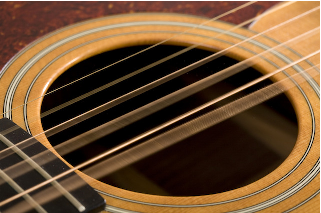
\includegraphics[width=0.4\textwidth]{images/guitare.pdf} & 
		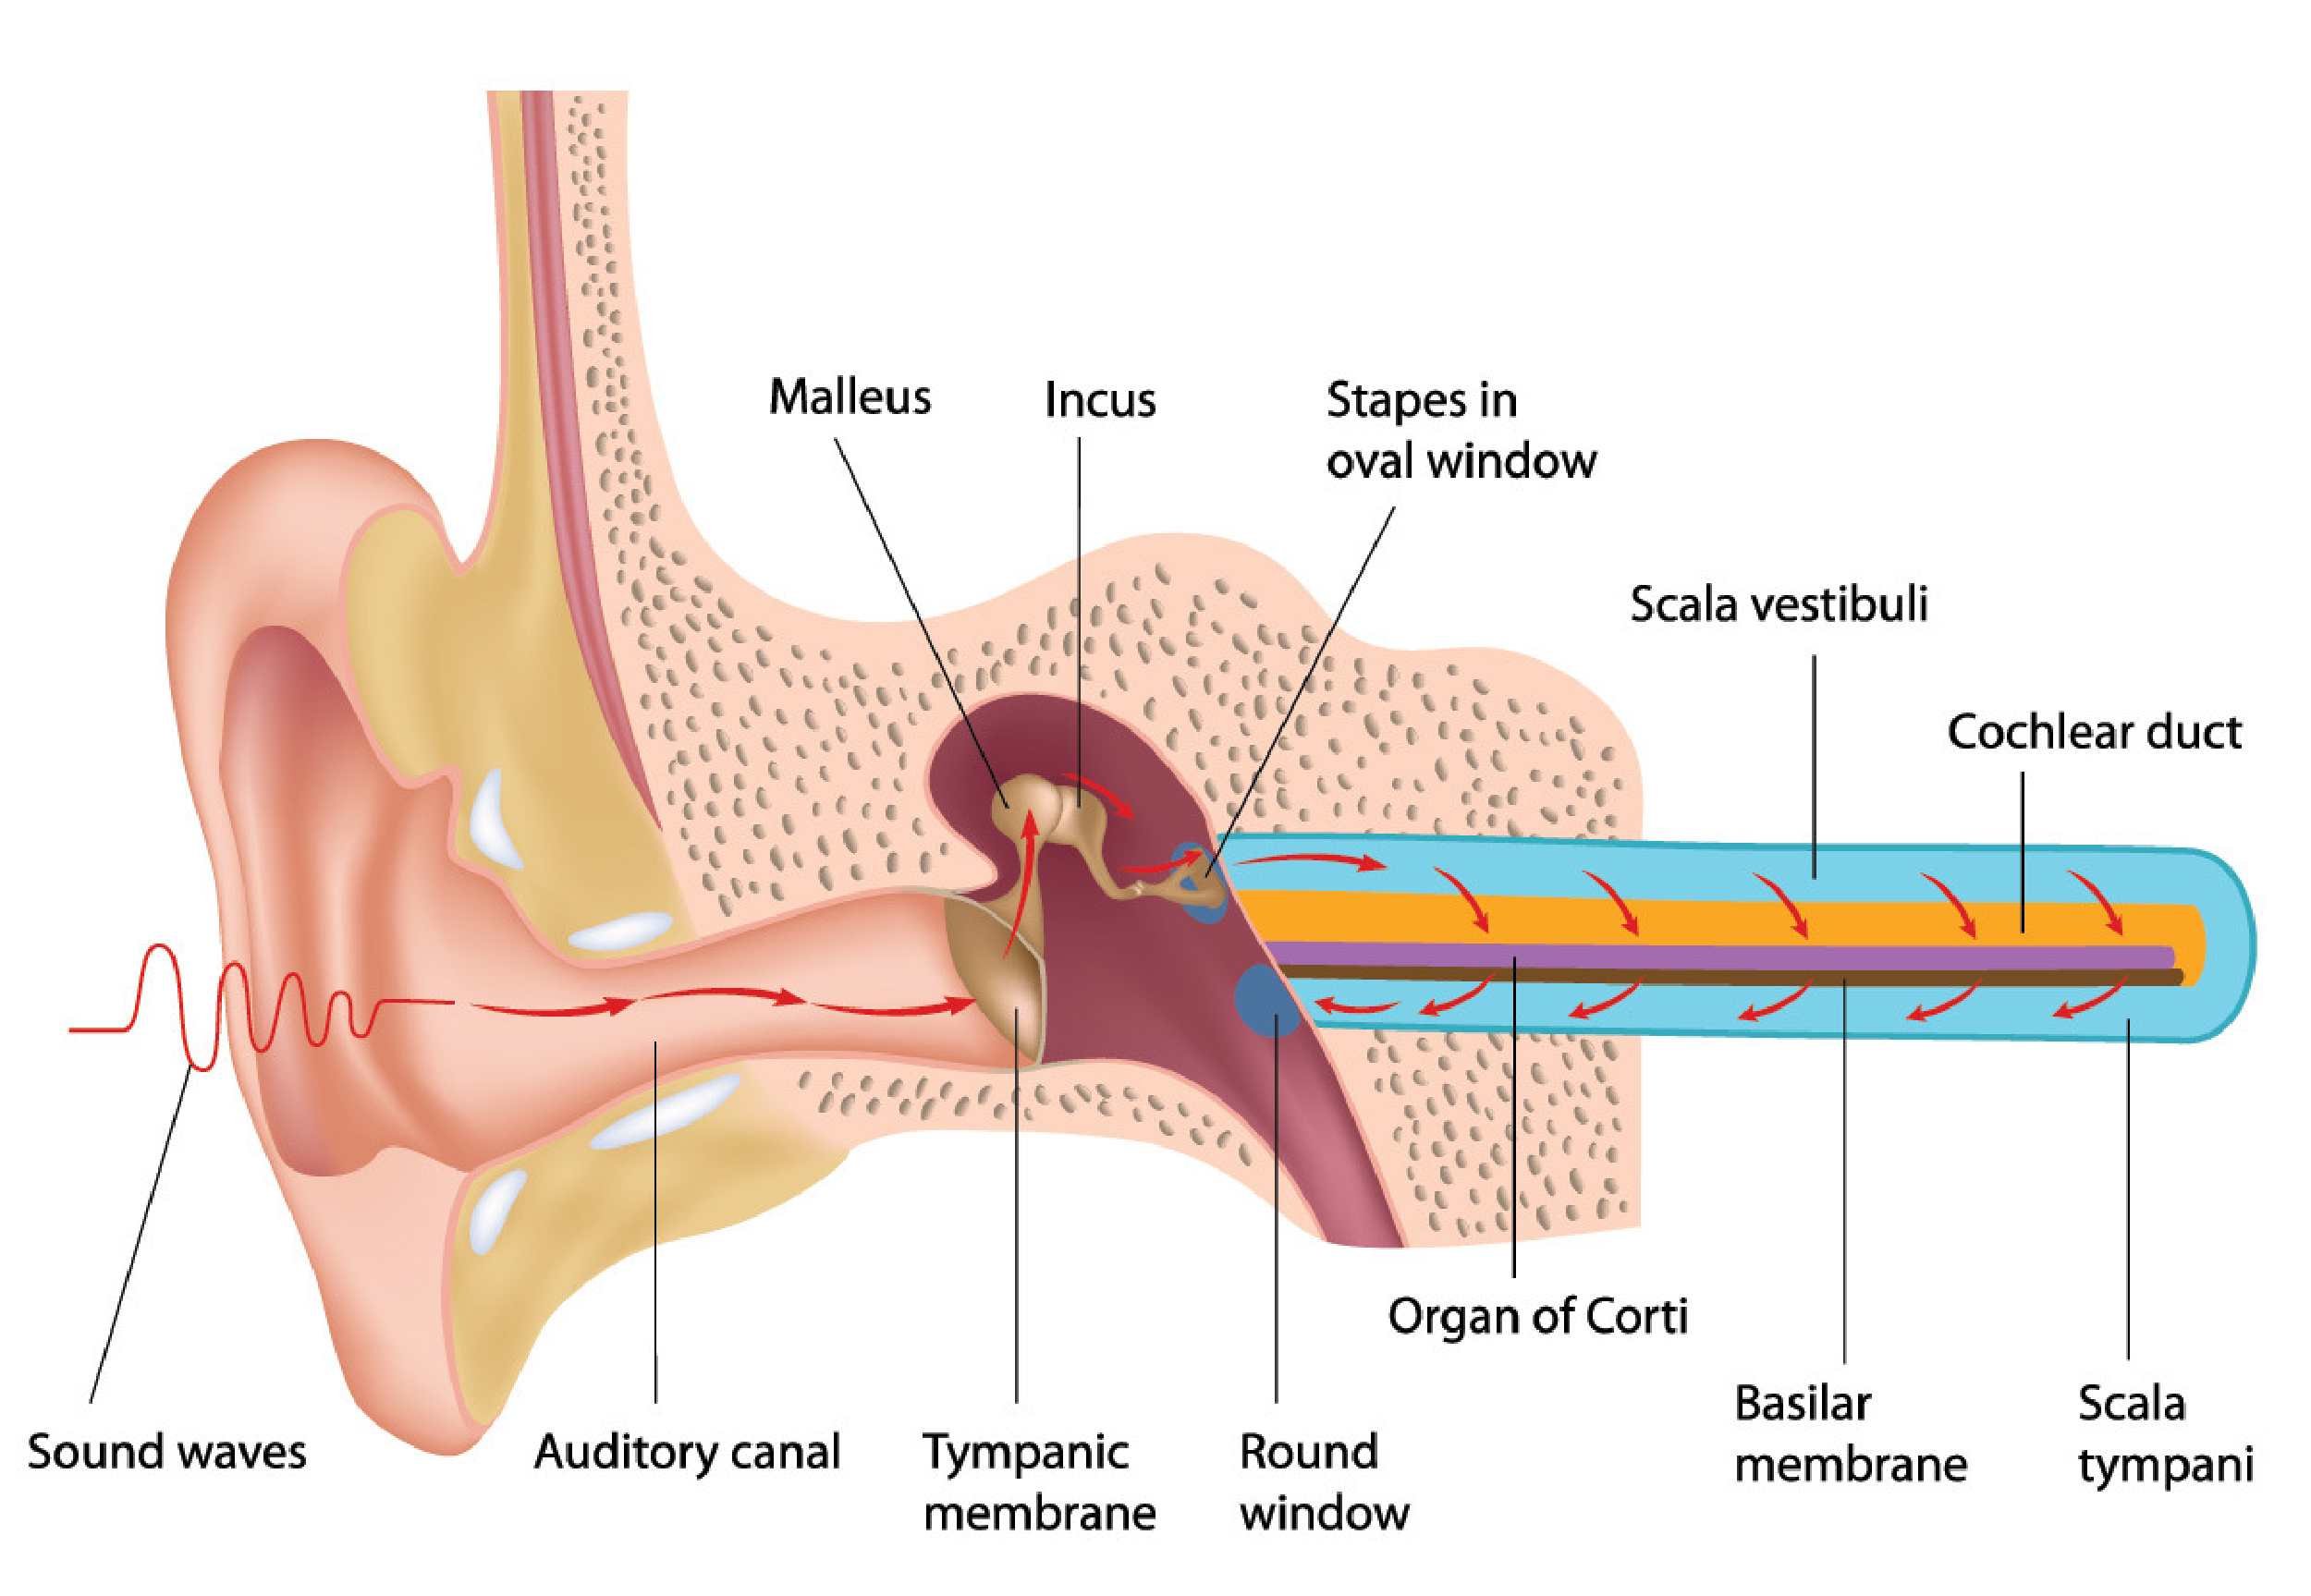
\includegraphics[width=0.4\textwidth]{images/oreille.pdf} 
	\end{tabular}
\end{center}

\section{\'Eléments pédagogiques}

\textbf{Objectifs}. L'objectif de ce TP est de vous faire manipuler certaines méthodes numériques étudiées en cours à travers une application acoustique, afin de vous sensibiliser aux difficultés de développement et de déploiement des outils numériques. Au terme de ce travail, vous aurez modélisé physiquement deux problèmes vibratoires (en 1D puis en 2D) et développé des méthodes numériques pour d'une part simuler le son d'une corde de guitare que vous pourrez écouter, et d'autre part de simuler et visualiser les vibrations de la membrane tympanique.
Ce TP sera réalisé par binôme uniquement. Vous programmerez dans l’environnement Scilab disponible sur les stations de travail de l'ENSIMAG et en téléchargement libre. Le TP fera l’objet d’un rapport précis, clair et concis mettant en avant les résultats obtenus ainsi que vos observations sur les méthodes utilisées. Il n'y a qu'un seul rapport à rendre par binôme.\\

\textbf{Organisation}. Une séance d'interactions concernant le TP est prévue. Nous vous invitons à venir préparer cette séance. Plus généralement, n'hésitez pas à demander des conseils, des précisions ou à poser vos questions par mail aux enseignants de TP. Le travail demandé dans ce TP est conséquent. Nous vous encourageons fortement à débuter le travail le plus tôt possible.\\

\textbf{Livrables}. Notez que ce sujet ne constitue que la base de ce qui vous est demandé : soyez critique par rapport à vos résultats, proposez d'autres idées, solutions ou tests. La mise en oeuvre de techniques de visualisation est fortement encouragée. La dernière page de votre compte-rendu devra être une sorte de manuel d'utilisation où vous expliquerez comment utiliser vos programmes. 
La lisibilité du code et la pertinence des commentaires seront pris en compte dans la note du TP. La qualité de la rédaction, de la synthèse, de l'analyse des résultats obtenus sont des critères importants pour la note. \\
Le TP est à rendre avant le 4 mai 2016 à 17h sous Teide, le livrable devra contenir : 
\begin{itemize}
	\item[$\bullet$] le compte rendu au format PDF (ne contenant pas de code !) 
	\item[$\bullet$] le code Scilab que vous avez utilisé 
	\item[$\bullet$] les images/animations qui mettent en valeur votre travail
\end{itemize}

 \newpage

%%%%%%%%%%%%%%%%%%%%%%%%%%%%%%%%%%%%%%%%%%%%%%%%%%%%%%%%
% 						                  	PARTIE I         
%%%%%%%%%%%%%%%%%%%%%%%%%%%%%%%%%%%%%%%%%%%%%%%%%%%%%%%%

\section*{Partie I : Modélisation et simulation d'une corde de guitare}

\subsection{Modélisation physique}

On considère une corde de guitare de longueur $L$ (en $m$), de masse linéique $\mu$ (en $kg.m^{-1}$) dont on applique une force tension $T$ (en Newton) aux extrémités d'où elle est fixée. \\

\indent $\blacksquare$ \textbf{Cas supposé sans raideur et de diamètre nul}\\

La corde initialement au repos occupe un segment le long de l'axe des $x$ (car on néglige l'effet de la pesanteur). On déforme la corde dans la direction perpendiculaire $y$ et on la lâche. Appelons $u(x,t)$ le déplacement de la corde à l'abscisse $x$ et à l'instant $t$. Ecrivons l'équation régie par la corde pour une portion de corde à l'aplomb du segment $[x,x +dx]$, de masse $dm$. Aux extrémités on a les forces $\vec{F_1}$ et $\vec{F_2}$ de module $T$ s'exerçant tangentiellement, comme sur la Figure \ref{fig:tension}.\\

Exprimons les forces $\vec{F_1}$ et $\vec{F_2}$ dans la base $(\vec{e_x},\vec{e_y})$ : 
\[ 
\overrightarrow{F_1} = - T (\cos \theta_1 \overrightarrow{e_x} + \sin \theta_1 \overrightarrow{e_y}), \quad \overrightarrow{F_2} = T (\cos \theta_2 \overrightarrow{e_x} + \sin \theta_2 \overrightarrow{e_y})
\]
 
En considérant les angles $\theta_1$ et $\theta_2$ petits, on a $\cos(\theta_i)\simeq 1$ et $\sin(\theta_i)\simeq \tan(\theta_i)\simeq \frac{\partial u}{\partial x}$ donc 
\[
\overrightarrow{F_1} = - T \left(\overrightarrow{e_x} + {\partial u \over \partial x} (x,t) \overrightarrow{e_y}\right), \quad 
\overrightarrow{F_2} = + T \left(\overrightarrow{e_x} + {\partial u \over \partial x} (x+\mathrm dx,t)\overrightarrow{e_y}\right)
\]

d'où 
\[ 
\overrightarrow{F_2} + \overrightarrow{F_1} \simeq 
T \left( {\partial u \over \partial x} (x+\mathrm dx,t) - {\partial u \over \partial x} (x,t)\right) \overrightarrow{e_y}\simeq 
T {\partial ^2 u \over \partial x^2 } (x,t) \mathrm d x \overrightarrow{e_y}
\]
 
Par ailleurs en utilisant la seconde loi de Newton qui relie la somme des forces à l'accélération  
\[ 
\vec{F_1}+\vec{F_2}=dm\frac{\partial ^2u}{\partial t^2}(x,t)\vec{e_y}=\mu dx\frac{\partial ^2u}{\partial t^2}(x,t)\vec{e_y}
\]
 
Ainsi en projetant sur $\vec{e_y}$, la corde est régie par l'équation des ondes 
\begin{equation}
	\frac{\partial ^2u}{\partial t^2}=\gamma^2\frac{\partial ^2u}{\partial x^2}
	\label{eq:ondes}
\end{equation}

avec $\gamma=\sqrt{\frac{T}{\mu}}$, la vitesse de propagation de l'onde.\\

\begin{figure}[b]
	\begin{center}
		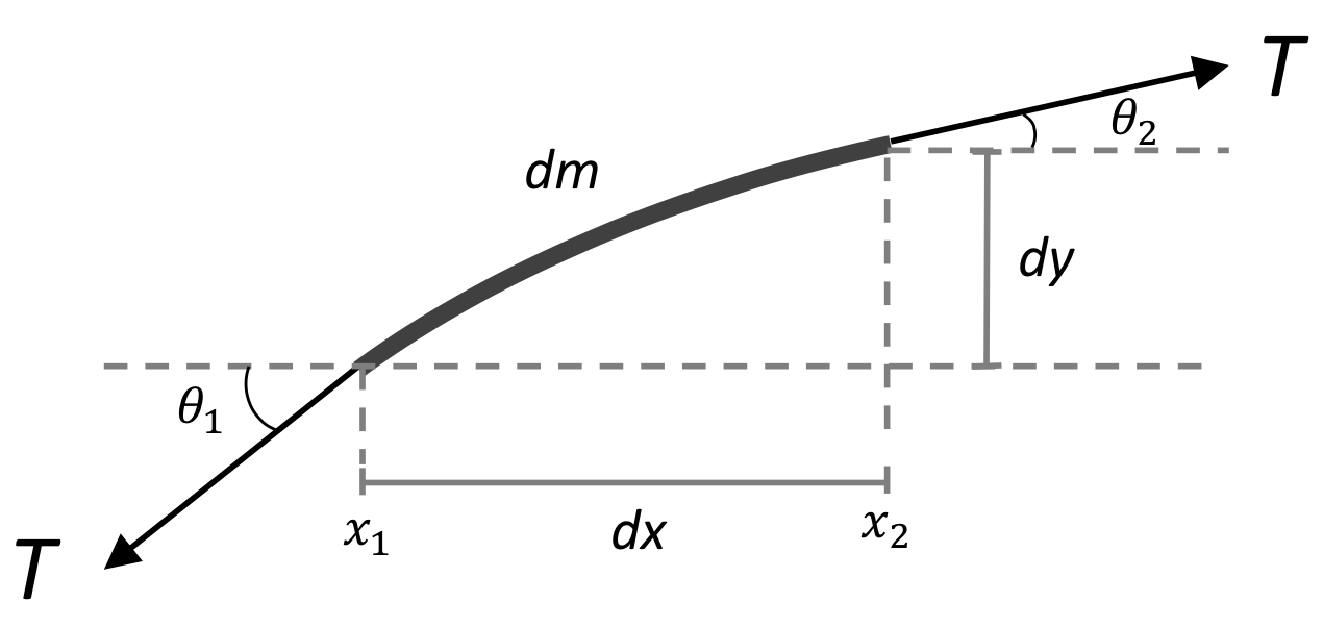
\includegraphics[width=0.7\textwidth]{images/tension.pdf}
		\caption{Forces de tension s'exerçant aux extrémités d'une portion de corde infinitésimale}
		\label{fig:tension}
	\end{center}
\end{figure}

\indent $\blacksquare$ \textbf{Modes propres de la vibration d'une corde}\\

%--- Question 1 ---%

\begin{mdframed}[style=exampledefault]
\question On cherche une solution de l'équation (\ref{eq:ondes}) sous la forme $u(x,t)=U(x)\cos(\omega t)$. Les conditions aux limites étant $u(0,t)=u(L,t)=0$, montrer qu'on obtient une famille de solutions 
\[
U_n(x)=B_n\sin\left(n\pi \frac{x}{L}\right),\quad \omega_n=n\pi \frac{\gamma}{L}\Leftrightarrow f_n=n\frac{1}{2L}\sqrt{\frac{T}{\mu}}
\]

et donc par le principe de superposition que $u$ s'écrit comme somme de tous les modes propres 
\[
u(x,t)=\sum_{n=1}^{+\infty}B_n\sin\left(n\pi \frac{x}{L}\right) \cos\left(n\pi \frac{\gamma t}{L}\right)
\]
avec 
\[ 
B_n = {2 \over L} \int_{0}^{L} u(x,0) \sin \left(n \pi {x \over L}\right) dx
\]

Comment varie la fréquence fondamentale $f_1$ (donc la note entendue) quand la longueur de la corde augmente? quand la longueur est divisée par 2? quand la masse linéique diminue? quand la tension augmente?
\end{mdframed}

%--- Fin Question 1 ---%

\indent $\blacksquare$ \textbf{Cas de la corde réelle avec raideur et amortissements}\\

La corde réelle est régie par l'équation aux dérivées partielles suivante :

\begin{equation} 
\left\{
	\begin{array}{l}
		\displaystyle \frac{\partial^2 u}{\partial t^2}=\gamma^2 \frac{\partial^2 u}{\partial x^2}-\kappa^2  				\frac{\partial^4 u}{\partial x^4}-2\sigma_0  \frac{\partial u}{\partial t}+2\sigma_1  \frac{\partial^3 u}{\partial t		\partial x^2}\\ \\ 
		\displaystyle u(0,t)=u(L,t)=\frac{\partial^2 u}{\partial x^2}(0,t)=\frac{\partial^2 u}{\partial x^2}(L,t)=0\\ \\  		\displaystyle u(x,0)=u_0(x), \quad \frac{\partial u}{\partial t}(x,0)=v_0(x)
	\end{array}
\right. 
\label{eq:model_stiff}
\end{equation}

$\bullet$ $\displaystyle -2\sigma_0  \frac{\partial u}{\partial t}$ est le terme d'amortissement du aux frottements de l'air, qui tend à ramener à la corde dans sa position d'équilibre. Cette force de résistance dépend de la longueur de la corde $L$, de la vitesse de propagation de l'onde $\gamma$ et du spectre de fréquence.\\

$\bullet$ $\displaystyle2\sigma_1  \frac{\partial^3 u}{\partial t\partial x^2}$ regroupe les termes de résistances internes et de processus dissipatifs induits par les propriétés intrinsèques du matériel, transformant l'énergie cinétique en énergie thermique, et donc contribuant également à ramener la corde à l'état d'équilibre.\\

$\bullet$ $\displaystyle-\kappa^2  \frac{\partial^4 u}{\partial x^4}$ est le terme de raideur qui dépend aussi du matériel qui compose la corde. En effet dans l'équation classique des ondes (\ref{eq:ondes}) on considérait la corde parfaitement flexible, mais en réalité il faut une certaine force pour courber la corde (quantifier par ce que l'on appelle le module de Young $E$). Le coefficient de raideur $\kappa$ a pour effet d'affecter la répartition des harmoniques 
\[
f_n = n \sqrt{1 + B n^2}f_1,\quad f_1=\frac{1}{2 L} \sqrt{\frac{T}{\mu}}
\]
en espaçant davantage les hautes fréquences, et par conséquent de modifier le timbre. Cet effet est quantifié via le paramètre d'inharmonicité $B$ exprimé par 
\[
B = \frac{\pi^3 E d^4}{64 T L^2}
\]
où $d$ est le diamètre de la corde, et le coefficient de raideur s'exprime par : 
\[
\kappa^2=\frac{4f_1^2L^4B}{\pi^2}
\]

$\bullet$ Les conditions initiales imposent que la corde soit fixée aux deux extrémités $u(0,t)=u(L,t)=0$, tout en permettant une rotation autour de ces points d'attaches (dans le cas contraire on aurait par exemple $\frac{\partial u}{\partial x}(0,t)=0$) mais en contraignant les oscillations dans le plan vertical (imposé par les moments nuls $\frac{\partial^2 u}{\partial x^2}(0,t)=\frac{\partial^2 u}{\partial x^2}(L,t)=0$). La corde est pincée (donc déformée suivant la fonction $u_0(x)$) et lâchée à l'instant $t=0$ avec une certaine vitesse $v_0(x)$, ce qui la fera osciller au cours du temps comme sur la Figure \ref{fig:profil}. \\

\begin{figure}
	\begin{center}
		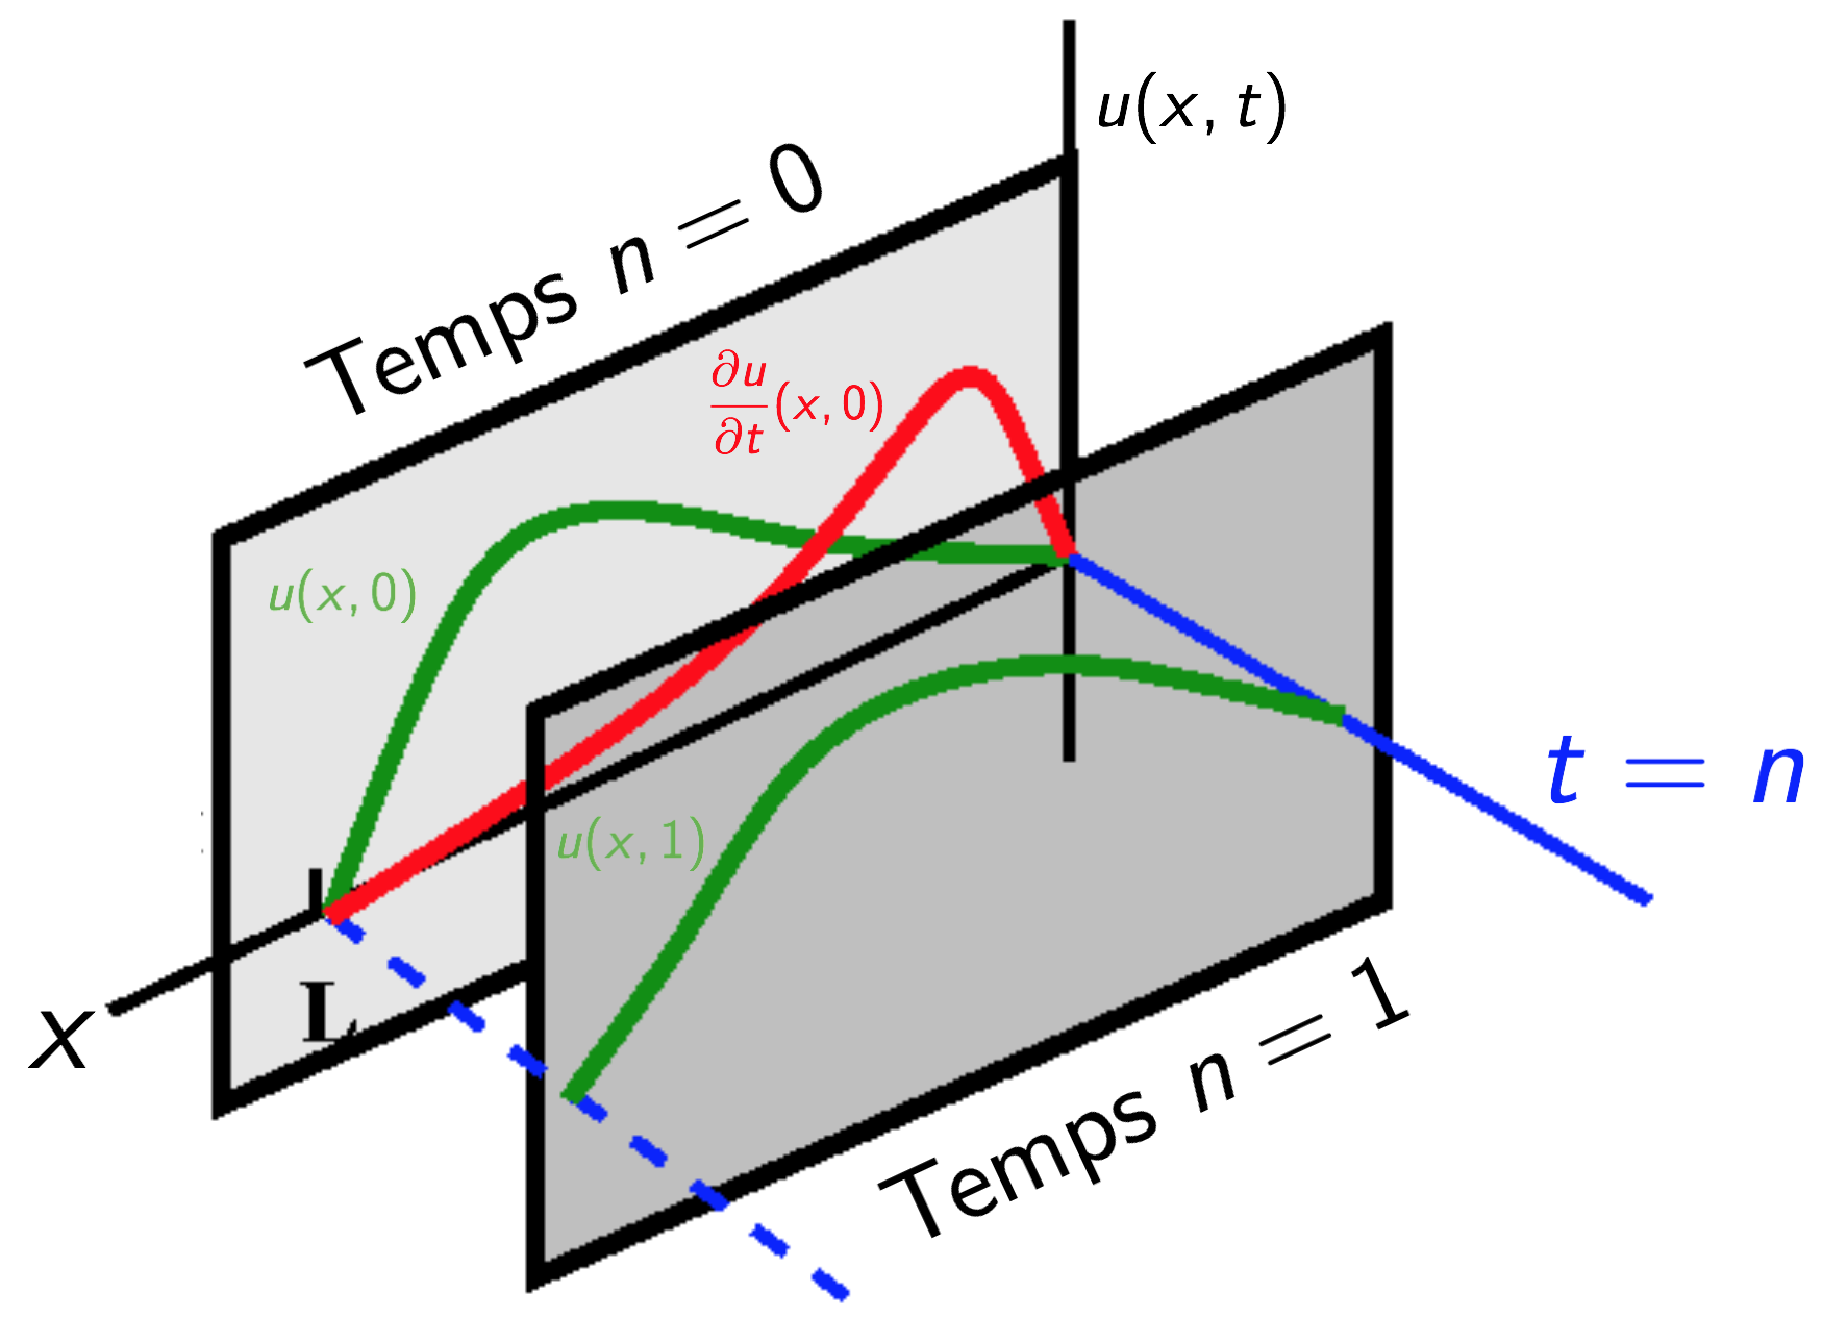
\includegraphics[width=0.9\textwidth]{images/profils_corde.pdf}
		\caption{Représentation de l'évolution du profil de la corde $x\mapsto u(x,t)$ à différents instants $t=n$}
		\label{fig:profil}
	\end{center}
\end{figure}

\textbf{En pratique}. On dispose des caractéristiques de la corde $L,d,T,E,\mu$ et on en déduit $f_1,B,\kappa$. Mais comme on préfère se donner la fréquence d'une note $f_1$, on dit que la longueur $L=1$ est fixée, $\mu$ également fixée à une valeur donnée (choix de la corde) et c'est donc la tension $T$ qui permet d'accorder sur la note désirée, ce qui permet de travailler sur une corde de longueur fixée pour notre choix de discrétisation. Finalement les deux paramètres du modèle $\kappa$ et $\gamma$ se déduisent des paramètres physiques $f_1$ et $B$ par : 
\[
\kappa=\frac{2f_1 \sqrt{B}}{\pi}, \quad \gamma=2f_1
\]

\subsection{Discrétisation du modèle par différences finies}

Discrétisons la corde de longueur $L=1$ en $N+1$ positions $x_l=lh$ avec $0\leqslant i\leqslant N$ et $h=\frac{1}{N}$, et le temps en $NF$ instants $t_n=nk$ avec $k=\frac{1}{SR}$ (où SR est le taux d'échantillonnage, typiquement 44100 Hz). Ainsi on approche la fonction continue $u(x,t)$ par $u_l^n$ en la position $x_l=lh$ et au temps $t_n=nk$, soit $u(x_l,t_n)=u(lh,nk)\approx u_l^n$. La grille de discrétisation est représentée Figure \ref{fig:grille}. \\

\begin{figure}
	\begin{center}
		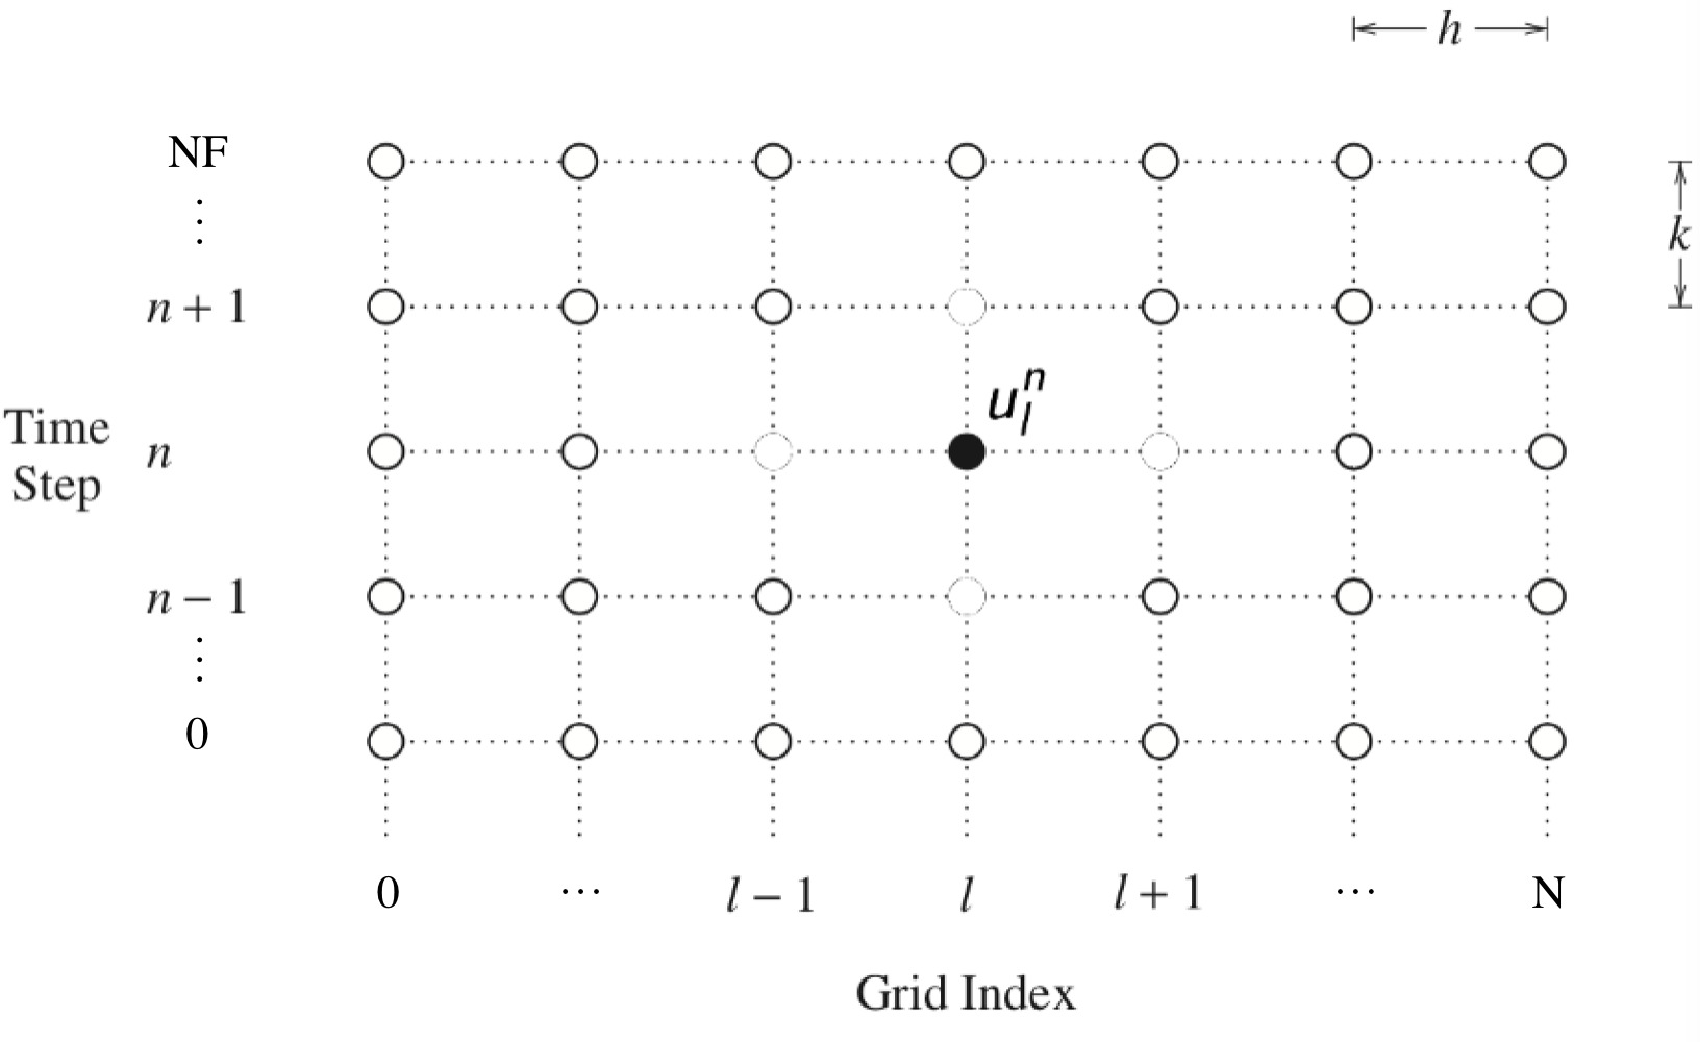
\includegraphics[width=0.9\textwidth]{images/grille.pdf}
		\caption{Grille de discrétisation en temps et en espace }
		\label{fig:grille}
	\end{center}
\end{figure}

On rappelle les formules Taylor à l'ordre 4 suivant la variable $x$ et $t$ : 
\[
u(x+h,t)=u(x,t)+h\frac{\partial u}{\partial x}(x,t)+\frac{h^2}{2!}\frac{\partial^2 u}{\partial x^2}(x,t)+\frac{h^3}{3!}\frac{\partial^3 u}{\partial x^3}(x,t)+\frac{h^4}{4!}\frac{\partial^4 u}{\partial x^4}(x,t)+o(h^4)
\]

\[
u(x,t+k)=u(x,t)+k\frac{\partial u}{\partial t}(x,t)+\frac{k^2}{2!}\frac{\partial^2 u}{\partial t^2}(x,t)+\frac{k^3}{3!}\frac{\partial^3 u}{\partial t^3}(x,t)+\frac{k^4}{4!}\frac{\partial^4 u}{\partial t^4}(x,t)+o(k^4)
\]

%--- Question 2 ---%

\begin{mdframed}[style=exampledefault]
\question En calculant $u(x+h,t)+u(x-h,t)$ (resp. $u(x,t+k)+u(x,t-k)$) montrer comme dans le cours que 

\begin{equation}
	\frac{\partial^2 u}{\partial x^2}(x,t)=\frac{u(x+h,t)-2u(x,t)+u(x-h,t)}{h^2}+o(1)
	\label{eq:taylor}
\end{equation}
 
et donc
\[
\begin{array}{l}
	\displaystyle \frac{\partial^2 u}{\partial x^2}(x_l,t_k)\approx \frac{1}{h^2}(u_{l+1}^n-2u_l^n+u_{l-1}^n)\\ \\ 		\displaystyle \frac{\partial^2 u}{\partial t^2}(x_l,t_k)\approx \frac{1}{k^2}(u_{l}^{n+1}-2u_l^n+u_{l}^{n-1})\end{array}
\]
 
De même en calculant $u(x+2h,t)+u(x-2h,t)-4[u(x+h,t)+u(x-h,t)]+6u(x,t)$ montrer 
\[
\frac{\partial^4 u}{\partial x^4}(x_l,t_k)\approx \frac{1}{h^4}(u_{l+2}^n-4u_{l+1}^n+6u_l^n-4u_{l-1}^n+u_{l-2}^n)
\]
 
En dérivant chaque terme de la relation (\ref{eq:taylor}) grâce au fait que 
\[
\frac{\partial u}{\partial t}(x,t)=\frac{u(x,t+k)-u(x,t-k)}{2k}+o(1)
\]
montrer que 
\[
\frac{\partial}{\partial t}\left(\frac{\partial^2 u}{\partial x^2}\right)\approx \frac{1}{2kh^2}(u_{l+1}^{n+1}-2u_{l}^{n+1}+u_{l-1}^{n+1}-u_{l+1}^{n-1}+2u_l^{n-1}-u_{l-1}^{n-1})
\]
 
En déduire que le schéma implicite associé à l'EDP (\ref{eq:model_stiff}) est 
\begin{align}
	&~~a_1u_{l-1}^{n+1}+a_2u_l^{n+1}+a_1u_{l+1}^{n+1}\\
	+& ~~b_1u_{l-2}^n+b_2u_{l-1}^n+b_3u_l^n+b_2u_{l+1}^n+b_1u_{l+2}^n\\ 
	+&~~ c_1u_{l-1}^{n-1}+c_2u_l^{n-1}+c_1u_{l+1}^{n-1}\\ 
	=&~0
\end{align}

avec 
\[ 
a_1=-\frac{\sigma_1 k}{h^2},\quad a_2=1+\sigma_0 k+\frac{2\sigma_1 k}{h^2}, 
\quad c_1=\frac{\sigma_1 k}{h^2},\quad c_2=1-\sigma_0 k-\frac{2\sigma_1 k}{h^2}
\]
\[
b_1=\frac{\kappa^2 k^2}{h^4}, \quad b_2=-\frac{\gamma^2 k^2}{h^2}-\frac{4\kappa^2 k^2}{h^4},
\quad b_3=-2+\frac{2\gamma^2 k^2}{h^2}+\frac{6\kappa^2 k^2}{h^4}
\]
\end{mdframed}

%--- Fin Question 2 ---%

Les voisins considérés sont ainsi représentés Figure \ref{fig:grid_neighbor}. On constate alors qu'il n'y a pas de problème d'indices pour les points $l\in [2,N-2]\cap \N$, ni pour $l=0$ et $l=N$ car la corde étant fixée aux extrémités on a par hypothèse $\forall n, u_0^n=u_N^n=0$. En revanche pour $l=1$ et $l=N-1$ on obtient respectivement $l-2=-1$ et $l+2=N+1$, on a donc besoin d'introduire des points dits \enquote{fantômes} ou \enquote{virtuels}, qu'on désigne par $u_{-1}^n$ et $u_{N+1}^n$.\\

Par la suite on désignera par $\overline{\ub}^n$ le vecteur des points de discrétisation de la corde à $t=n$ 
\[
\overline{\ub}^n=\begin{bmatrix}u_0^n\\ u_1^n\\ \vdots \\ u_{N-1}^n \\ u_N^n\end{bmatrix}
\]

%--- Question 3 ---%

\begin{mdframed}[style=exampledefault]

\question Montrer en utilisant les conditions aux limites que $u_{-1}=-u_1$ et $u_{N+1}=-u_{N-1}$ puis que le schéma numérique peut s'écrire sous forme matricielle 
\begin{equation}
	\overline{\A} \overline{\ub}^{n+1}+\overline{\B} \overline{\ub}^n+\overline{\C} \overline{\ub}^{n-1}=0
\end{equation} 
avec les matrices de tailles $(N+1)\times (N+1)$ suivantes : 
\[
\overline{\A}=
\begin{bmatrix}
1 & 0 & 0 & 0 & \cdots & 0 \\ 
a_1 & a_2 & a_1 & 0 & \cdots & 0 \\ 
0 & a_1 & a_2 & a_1 & \ddots & 0 \\
\vdots & \ddots & \ddots & \ddots & \ddots & \vdots \\ 
0 & \cdots & 0 & a_1 & a_2 & a_1\\ 
0 & \cdots & 0 & 0 & 0 & 1 \\
\end{bmatrix},\quad 
\overline{\C}=
\begin{bmatrix}
1 & 0 & 0 & 0 & \cdots & 0 \\ 
c_1 & c_2 & c_1 & 0 & \cdots & 0 \\
0 & c_1 & c_2 & c_1 & \ddots & 0 \\ 
\vdots & \ddots & \ddots & \ddots & \ddots & \vdots \\
0 & \cdots & 0 & c_1 & c_2 & c_1 \\
0 & \cdots & 0 & 0 & 0 & 1 \\
\end{bmatrix},
\]
\[ 
\overline{\B}=
\begin{bmatrix}
1 & 0 & 0 & 0 & 0  & \cdots & 0 \\ 
b_2 & b_3-b_1 & b_2 & b_1 & 0 & \cdots & 0 \\ 
b_1 & b_2 & b_3 & b_2 & b_1 & \ddots & 0 \\
\vdots & \ddots & \ddots & \ddots & \ddots & \ddots & \vdots \\ 
0 & \cdots & b_1 & b_2 & b_3 & b_2 & b_1 \\ 
0 & \cdots &  0 & b_1 & b_2 & b_3-b_1 & b_2 \\ 
0 & \cdots & 0 & 0 &  0 & 0 & 1 \\
\end{bmatrix}
\]
\end{mdframed}

%--- Fin Question 3 ---%

Notons que les $u_0^n$ et $u_{N}^n$ sont connus et valent zéro, on peut donc ne pas en tenir compte dans les calculs, ce qui revient à considérer le vecteur 
\[
\ub^n=\begin{bmatrix}u_1^n\\ \vdots \\ u_{N-1}^n\end{bmatrix}
\]
et les sous-matrices centrales de taille $(N-1)\times (N-1)$ : $\A$, $\B$ et $\C$ respectivement de $\overline{\A}$, $\overline{\B}$ et $\overline{\C}$, pour lesquelles on a supprimé la première et dernière ligne et colonne, à savoir :

\[
\A=
\begin{bmatrix} 
a_2 & a_1 & 0 & \cdots & 0 \\ 
a_1 & a_2 & a_1 & \ddots & \vdots \\ 
0 & a_1 & a_2 & \ddots  & 0 \\ 
\vdots & \ddots & \ddots & \ddots  & a_1 \\ 
0 & \cdots & 0 & a_1 & a_2  \\
\end{bmatrix},\quad 
\C=
\begin{bmatrix} 
c_2 & c_1 & 0 & \cdots & 0 \\ 
c_1 & c_2 & c_1 & \ddots & \vdots \\ 
0 & c_1 & c_2 & \ddots  & 0 \\ 
\vdots & \ddots & \ddots & \ddots  & c_1 \\ 
0 & \cdots & 0 & c_1 & c_2  \\
\end{bmatrix},
\]
\[
\B=
\begin{bmatrix}
b_3-b_1 & b_2 & b_1 & 0 & \cdots & 0  \\ 
b_2 & b_3 & b_2 & b_1 & \ddots & \vdots \\  
b_1 & b_2 & b_3 & b_2 & \ddots & 0 \\ 
0 & \ddots & \ddots & \ddots & \ddots &b_1\\ 
\vdots & \ddots & b_1 & b_2 & b_3 & b_2  \\ 
0 & \cdots &  0 & b_1 & b_2 & b_3-b_1  \\
\end{bmatrix}
\]

On définit la matrice Toeplitz suivante et son carré : 
\[
\D_{xx}=\frac{1}{h^2}
\begin{bmatrix}
\ddots & \ddots & & & & \mathbf{0}  & \\
\ddots & -2 & 1 & & & & \\ 
& 1 & -2 & 1 & & & \\ 
& & 1 & -2 & 1 & & \\ 
& & & 1 & -2 & \ddots \\ 
& \mathbf{0} & & & \ddots & \ddots
\end{bmatrix}, 
\quad \D_{xxxx}=\D_{xx}\D_{xx}
\]

%--- Question 4 ---%

\begin{mdframed}[style=exampledefault]
\question Montrer que $$\A=(1+\sigma_0 k)\mathbf{I}-\sigma_1 k \D_{xx}, \quad \B=-2\mathbf{I}-\gamma^2 k^2 \D_{xx}+\kappa^2 k^2\D_{xxxx}, \quad \C=(1-\sigma_0 k)\mathbf{I}+\sigma_1 k \D_{xx}$$
\end{mdframed}

%--- Fin Question 4 ---%

\hspace{0.5cm} $\blacksquare$ \textbf{Stabilité du schéma numérique} \\

Par une analyse de Von Neumann on montre que la condition de stabilité du schéma s'écrit 
\[
h\geqslant h_{min}=\sqrt{\frac{\gamma^2k^2+\sqrt{\gamma^4 k^4+16\kappa^2 k^2}}{2}}
\]

\begin{figure}
	\begin{center}
		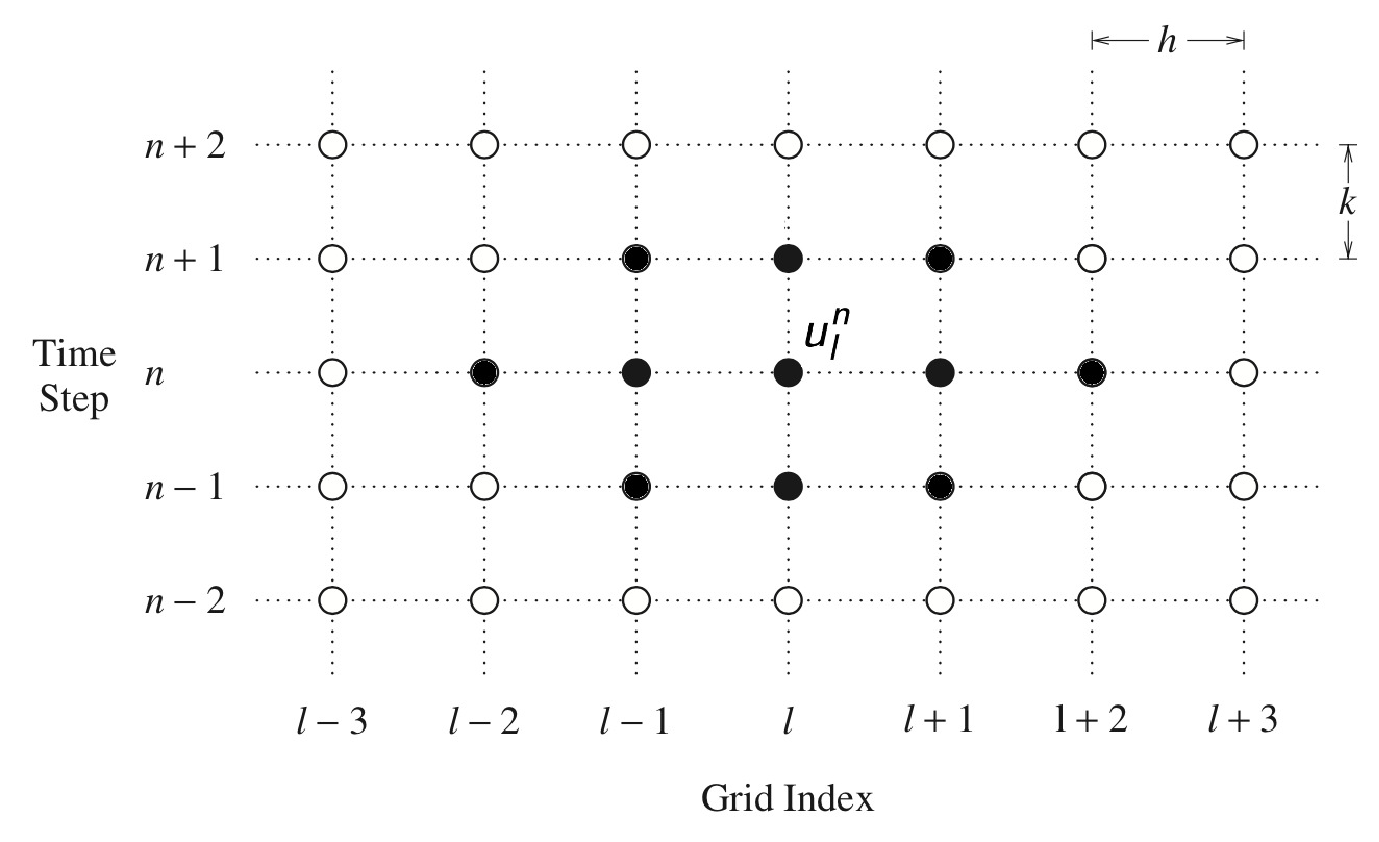
\includegraphics[width=0.7\textwidth]{images/grid_neighbor.pdf}
		\caption{Les voisins utilisés dans le schéma numériques }
		\label{fig:grid_neighbor}
	\end{center}
\end{figure}

\subsection{Programmation du schéma implicite sous Scilab}

\hspace{0.5cm} $\blacksquare$ \textbf{Choix des paramètres} $\sigma_0$  \textbf{et}  $\sigma_1$\\

%--- Question 5 ---%

\begin{mdframed}[style=exampledefault]
\question Ecrire l'équation caractéristique de l'EDP (\ref{eq:model_stiff}) en y injectant $\tilde u(x,t)=e^{st+j\beta x}$, et montrer que pour $\sigma_0\geqslant 0$ et $\sigma_1\geqslant 0$ petits, ses racines sont données par $s_{\pm}=\sigma\pm j\omega$ où 
\[
\sigma(\beta)=-\sigma_0-\sigma_1\beta^2,\quad \omega(\beta)=\sqrt{\gamma^2 \beta^2+\kappa^2\beta^4-(\sigma_0+\sigma_1\beta^2)^2}
\]
Ainsi la perte $\sigma(\beta)$ décroît avec le nombre d'onde $\beta$, et vaut $-\sigma_0$ quand la raideur n'est pas prise en compte.  Montrer que $\sigma$ dépend de la fréquence $\omega$ où 
\[
\sigma(\omega)=-\sigma_0-\sigma_1\xi (\omega),\quad \xi(\omega)=\frac{-\gamma^2+\sqrt{\gamma^4+4\kappa^2 \omega^2}}{2\kappa^2}
\]
On note $T_{60}(\omega)$ la constante de décroissance dépendant de la fréquence $\omega$ et définie par 
\[
T_{60}(\omega)=-\frac{6\ln 10}{\sigma(\omega)}
\]
Montrer enfin que pour 2 fréquences données $\omega_1<\omega_2$ on a 
\[
\sigma_0=\frac{6 \ln 10}{\xi(\omega_2)-\xi(\omega_1)}\left(\frac{\xi(\omega_2)}{T_{60}(\omega_1)}-\frac{\xi(\omega_1)}{T_{60}(\omega_2)}\right), \quad \sigma_1=\frac{6 \ln 10}{\xi(\omega_2)-\xi(\omega_1)}\left(-\frac{1}{T_{60}(\omega_1)}+\frac{1}{T_{60}(\omega_2)}\right)
\]
\end{mdframed}

%--- Fin Question 5 ---%

On définira ainsi comme paramètre un vecteur de perte $loss=[\omega_1/2\pi,T_{60}(\omega_1) ; \omega_2/2\pi,T_{60}(\omega_2)]$ servant à calculer $\sigma_0$ et $\sigma_1$. \\

\hspace{0.5cm} $\blacksquare$ \textbf{Conditions initiales} $u_0(x)$ \textbf{et} $v_0(x)$\\

A l'instant $t=0$ la corde est pincée à l'abscisse $x=x_0$ et étirée à la hauteur $c_0$, donc on considèrera $u(x,0)=u_0(x)$ une fonction triangle comme illustrée sur la Figure \ref{fig:triangle}. De plus on suppose que la corde est lâchée sans vitesse initiale donc $v_0(x)=0$.\\

\begin{figure}
	\begin{center}
		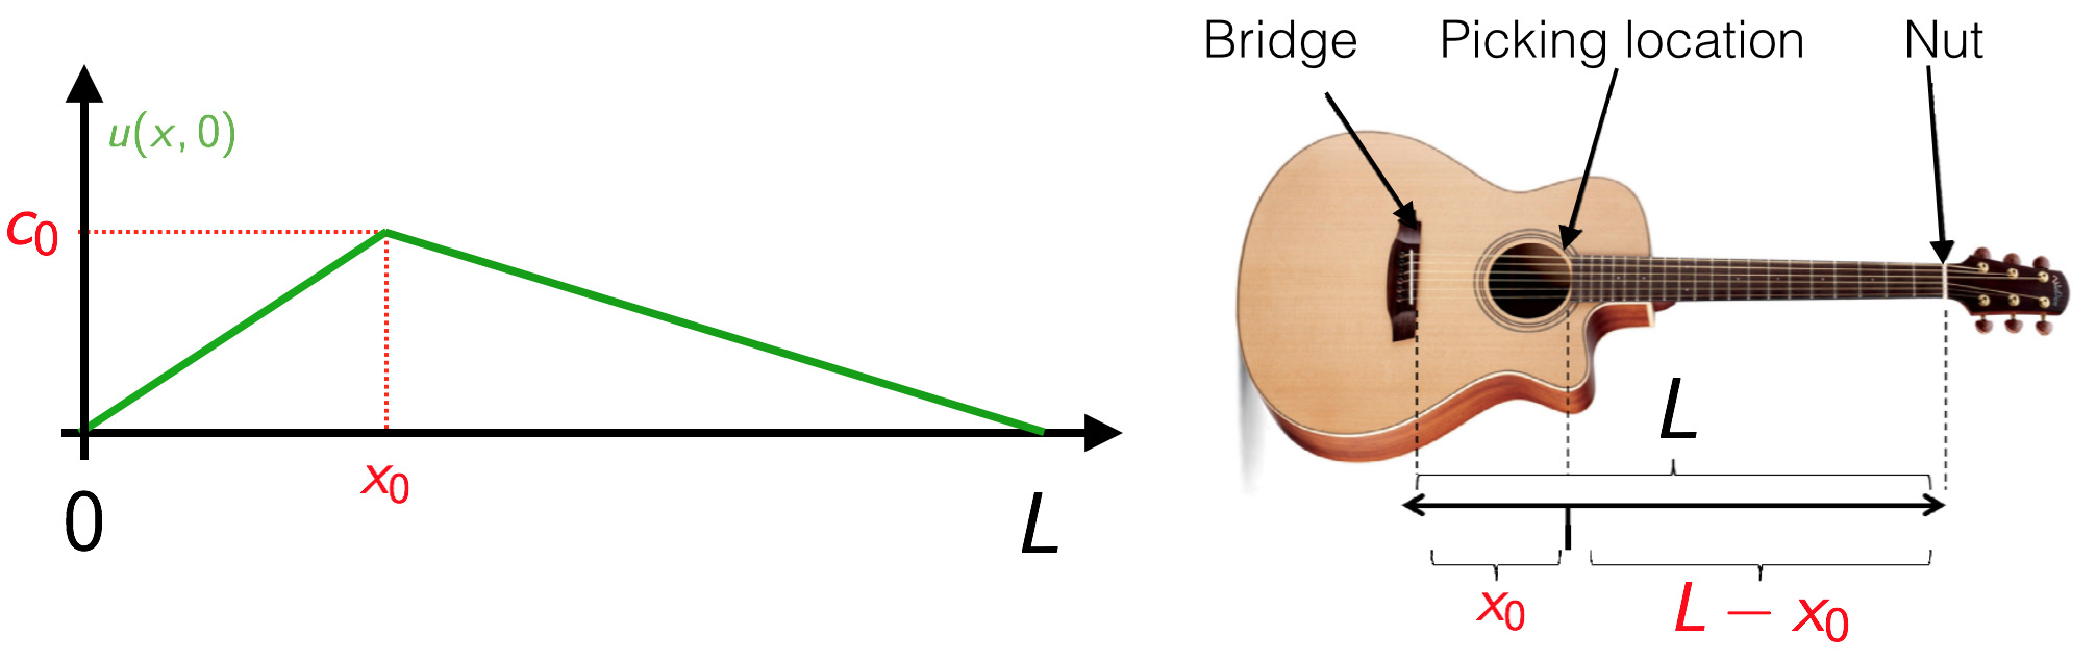
\includegraphics[width=\textwidth]{images/triangle.pdf}
		\caption{\'Etat initial de la corde $u(x,0)$ au moment du pincement $t=0$}
		\label{fig:triangle}
	\end{center}
\end{figure}

\hspace{0.5cm} $\blacksquare$ \textbf{Enregistrement stéréo et positionnement des micros}\\

La corde va ensuite osciller pour $t>0$ comme sur la Figure \ref{fig:profil}, et donc faire vibrer l'air par son déplacement et provoquer ainsi un son. Pour enregistrer ce son il faut donc être capable de mesurer les variations de déplacements de la corde, c'est le rôle des aimants placés sous les cordes qui génère par induction une force électromotrice dans une bobine sous l'action des vibrations de la corde modifiant ainsi le champ magnétique, comme expliqué Figure \ref{fig:micros2}. Ces aimants font donc office de micros, et sont disposés à différentes positions sur la guitare comme en témoigne la Figure \ref{fig:micros}. Dans notre simulation nous allons considérer 2 micros dont les deux positions au niveau de la corde sont données par le vecteur $rp=[p_1,p_2]$ (rp comme \textit{record position}). Le vecteur $out=zeros(2,NF)$ va donc enregistrer aux deux positions $p_1$ et $p_2$, toutes les hauteurs de déplacements $u(:,p_1)$ et $u(:,p_2)$ ($NF$ échantillons). Ces positions ne coïncidant pas forcément avec les points de discrétisation $x_i=ih$ il sera nécessaire de faire une interpolation linéaire.

\begin{figure}
	\begin{center}
		\begin{tabular}{cc}
			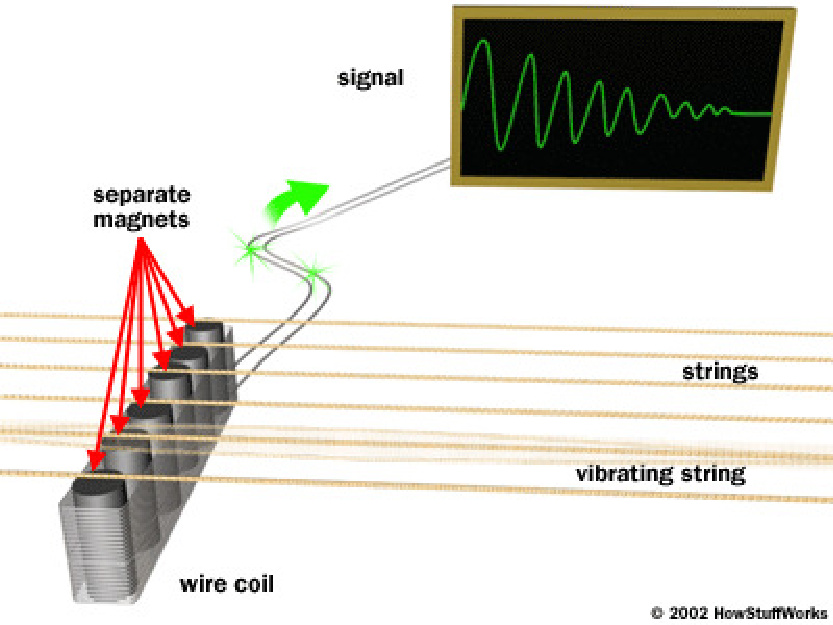
\includegraphics[width=0.5\textwidth]{images/micros_schema.pdf} &
			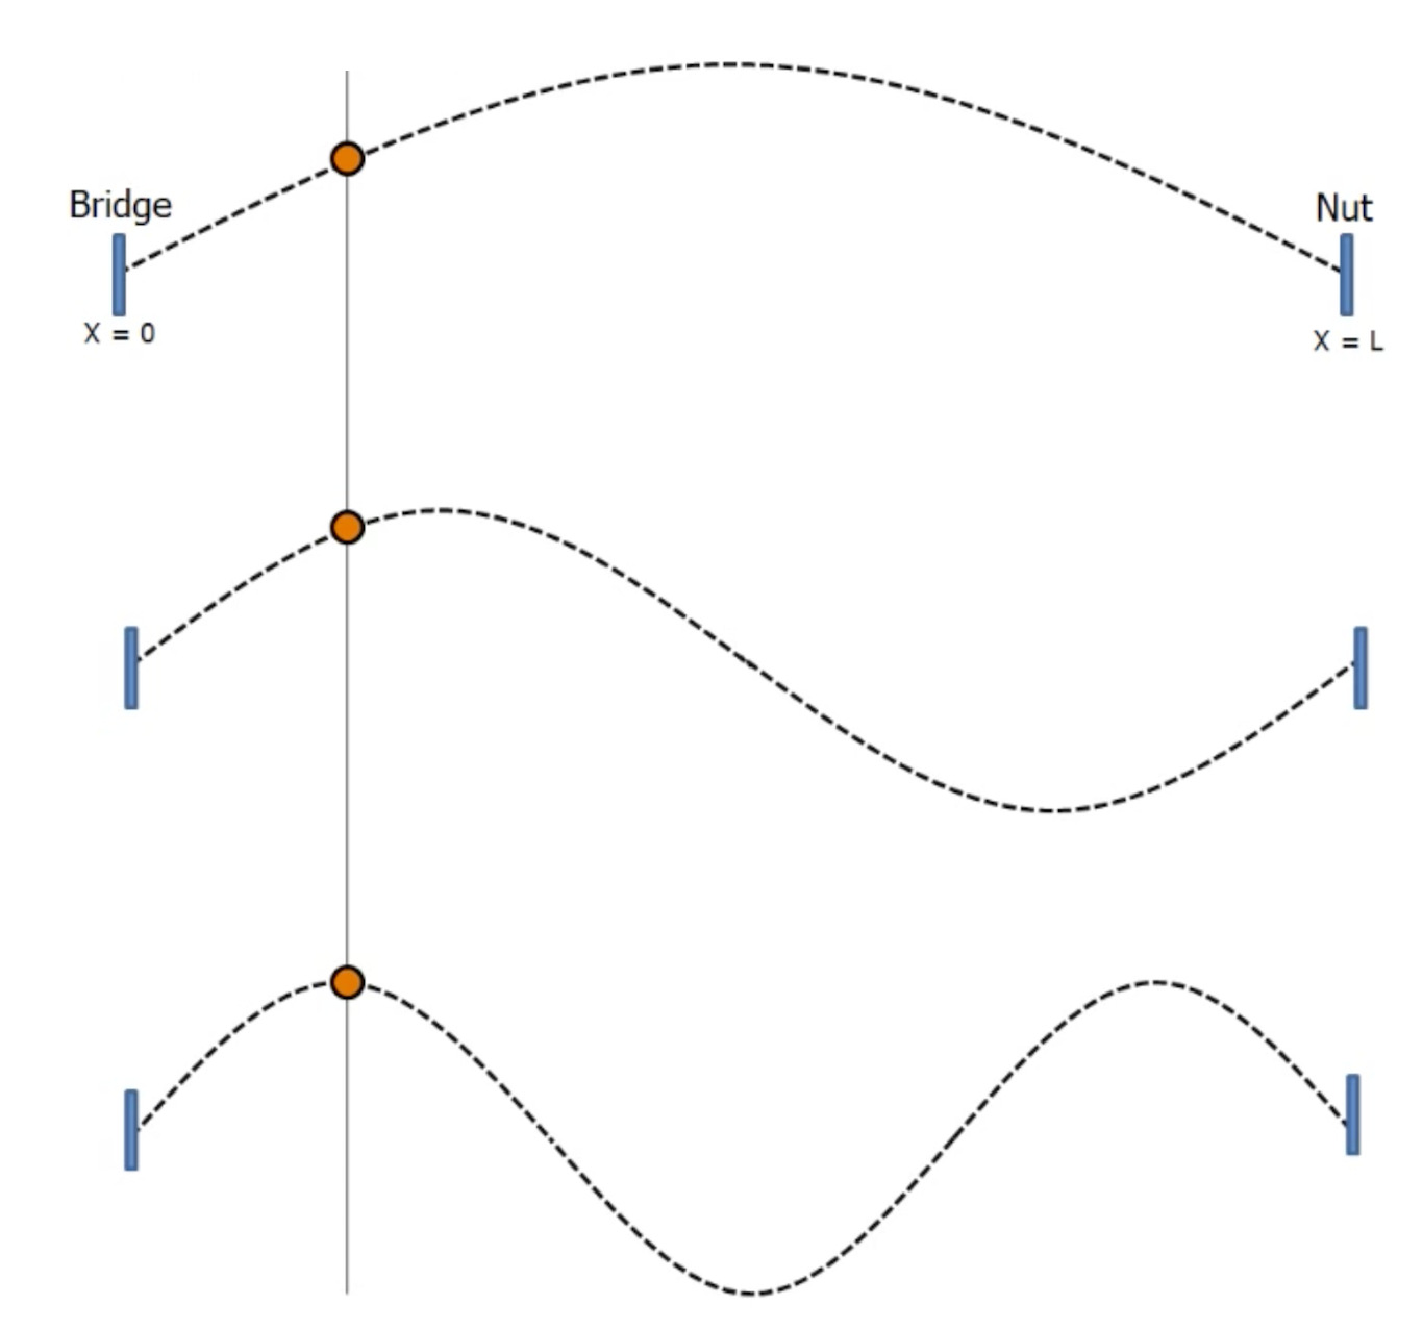
\includegraphics[width=0.5\textwidth]{images/micros_positions.pdf}
		\end{tabular}
		\caption{Sur le schéma de gauche chaque micro (composé d'un aimant) enregistre les déplacements 		d'une corde à une position donnée (point en orange sur le schéma de droite), donnant lieu à un signal 		sonore (en vert). En effet la corde métallique vibrant, celle-ci fait varier le circuit magnétique de l'aimant, 		ce qui génère par induction une force électromotrice dans la bobine, proportionnelle à la vitesse de 			déplacement de la corde.}
		\label{fig:micros2}
	\end{center}
\end{figure}

\begin{figure}
	\begin{center}
		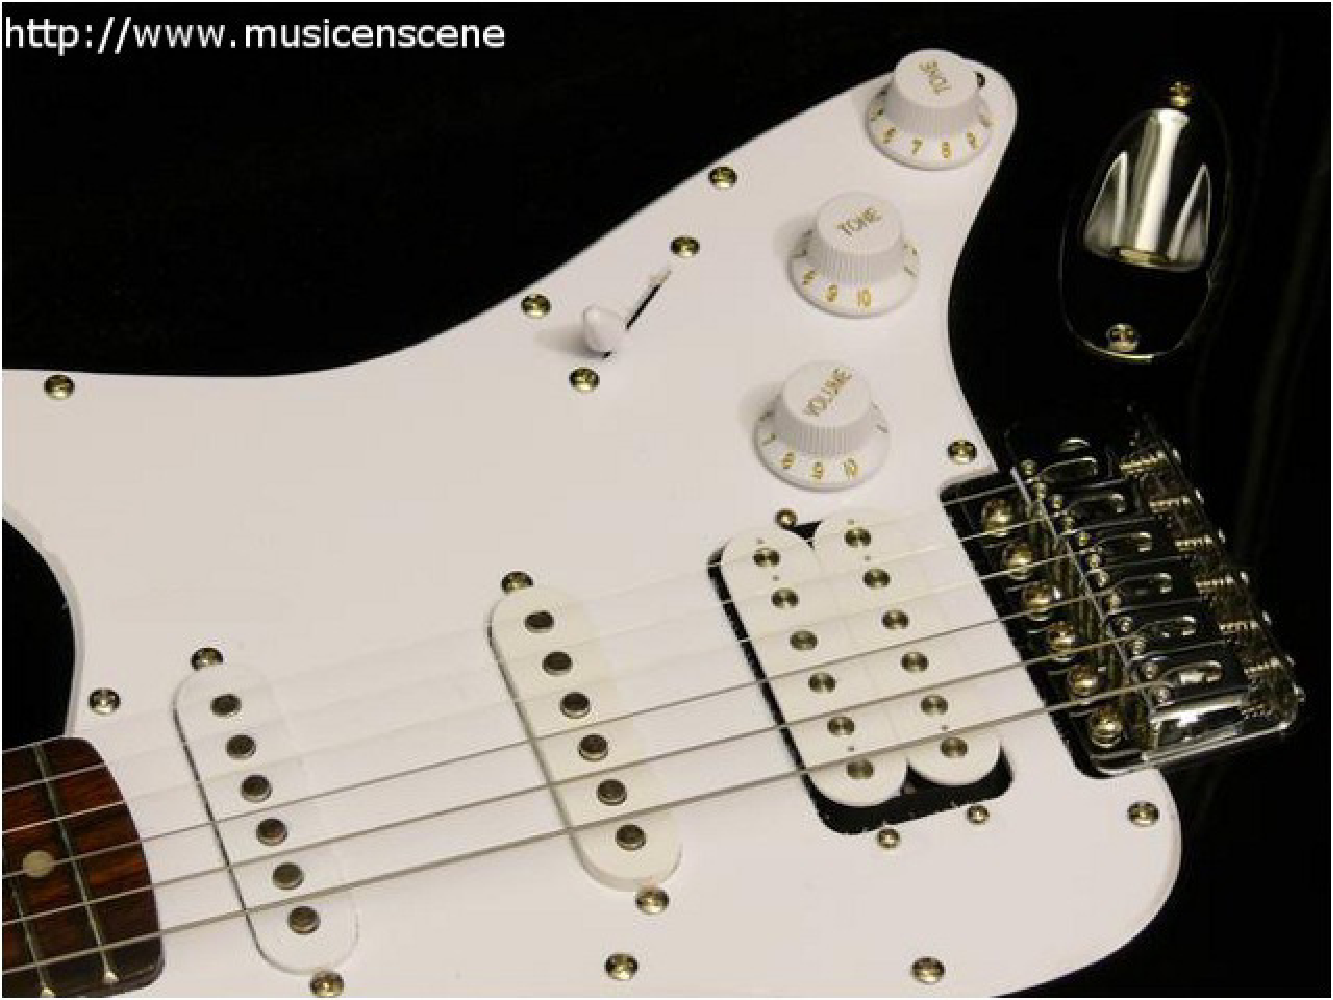
\includegraphics[scale=0.4,trim = 0mm 0mm 0mm 15mm,clip]{images/micros.pdf}
		\caption{Position des micros sur une guitare Fender Stratocaster comprenant un \textit{humbucker} 			(micro double bobinage) et deux micros simples.}
		\label{fig:micros}
	\end{center}
\end{figure}

\begin{lstlisting}[frame=single,caption=Paramètres d'entrée]  
start
SR = 44100;                  // taux d'échantillonage 
B = 0.001;                   // paramètre d'inharmonicité
f = 110;                     // fréquence fondamentale
TF = 4;			     // durée de la simulation
xo = 0.1;                    // position où la corde est pincée
co = 1;                      // hauteur du pincement
rp = [0.3 0.7];              // positions des micros
loss = [100, 10; 1000, 8];   // couples de fréquence/temps décroissance
\end{lstlisting}

%--- Question 6 ---%

\begin{mdframed}[style=exampledefault]
\question Ecrire un programme Scilab qui à partir des paramètres d'entrée fournis : \\

\begin{itemize}
	\item[$\bullet$] Calcule itérativement le profil de la corde (vecteurs $\ub^n$) tout en affichant l'animation\\
	\item[$\bullet$] Calcule et affiche le vecteur $out$ enregistrant les vibrations aux positions des micros $rp$\\ 	\item[$\bullet$] Emet le son de la corde en stereo à partir du vecteur $out$
\end{itemize}
\end{mdframed}

%--- Fin Question 6 ---%

Vous pourrez écrire les matrices $A,B,C$ directement via les commandes \verb"toeplitz" et \verb"sparse".
Pour une aide Scilab quant à la réalisation de l'animation et du son, se référer à l'annexe.

\subsection{Analyses qualitative et quantitative du son produit}

On commence par s'assurer que la note simulée correspond bien à la fréquence fondamentale en entrée. Par exemple pour $f=110~Hz$, la note LA, vous pouvez vérifier avec une vraie guitare ou encore en décrochant votre téléphone (la tonalité est un LA par défaut). Mais on se propose ici de le vérifier mathématiquement (après tout votre instrument est peut-être mal accordé). 

%--- Question 7 ---%

\begin{mdframed}[style=exampledefault]
\question Dans cette question on attend de vous que vous preniez du recul quant à vos résultats obtenus.\\

\begin{itemize}
	\item[$\bullet$] Calculer et afficher la transformée de Fourier du signal $s_1=out(:,1)$ via la commande $fft$ 	(la symétrie vous permet de ne garder qu'une partie du spectre, ou de repositionner correctement les 		fréquences autour de zéro via la commande $fftshift$). Déterminer l'indice auquel correspond le pic maximum 	du spectre. Cette fréquence fondamentale est bien celle que vous avez déclarée en entrée?\\ 
	\item[$\bullet$] \textbf{Quantitativement} quel est l'effet sur le spectre du paramètre d'inharmonicité $B$? de 	la position $x_0$ où l'on pince la corde (vers le centre ou près de l'attache appelée le chevalet) ? \\ 
	\item[$\bullet$] \textbf{Qualitativement} quels sont les effets de $B$ et $x_0$ sur le timbre du son joué?\end{itemize} 
\end{mdframed}

%--- Fin Question 7 ---%

Le son produit par la corde de la guitare se propage dans l'air jusqu'à l'oreille et vient frapper le tympan, membrane élastique, mince et résistante qui se déforme sous l'action de la pression de l'air et vibre à la même fréquence. La fonction du tympan est de faire passer l'information de l'extérieur (air puis oreille externe = milieu gazeux) à l'intérieur (oreille interne = milieu solide et liquide). Cette objectif est atteint grâce au trois osselets : marteau, enclume, étrier. Ce dernier étant en contact avec l'oreille interne. Le son actionne le marteau qui vient frapper l'enclume dont la base est relié à l'étrier. Le passage au travers du tympan va donc transformer les vibrations de l'air en vibrations mécaniques, puis enfin en l'information nerveuse grâce aux organes de Corti, que le cerveau se chargera d'interpréter. On se propose dans la partie suivante de modéliser la membrane tympanique en \enquote{oscillations libres}.

\begin{figure}[H]
	\begin{center}
		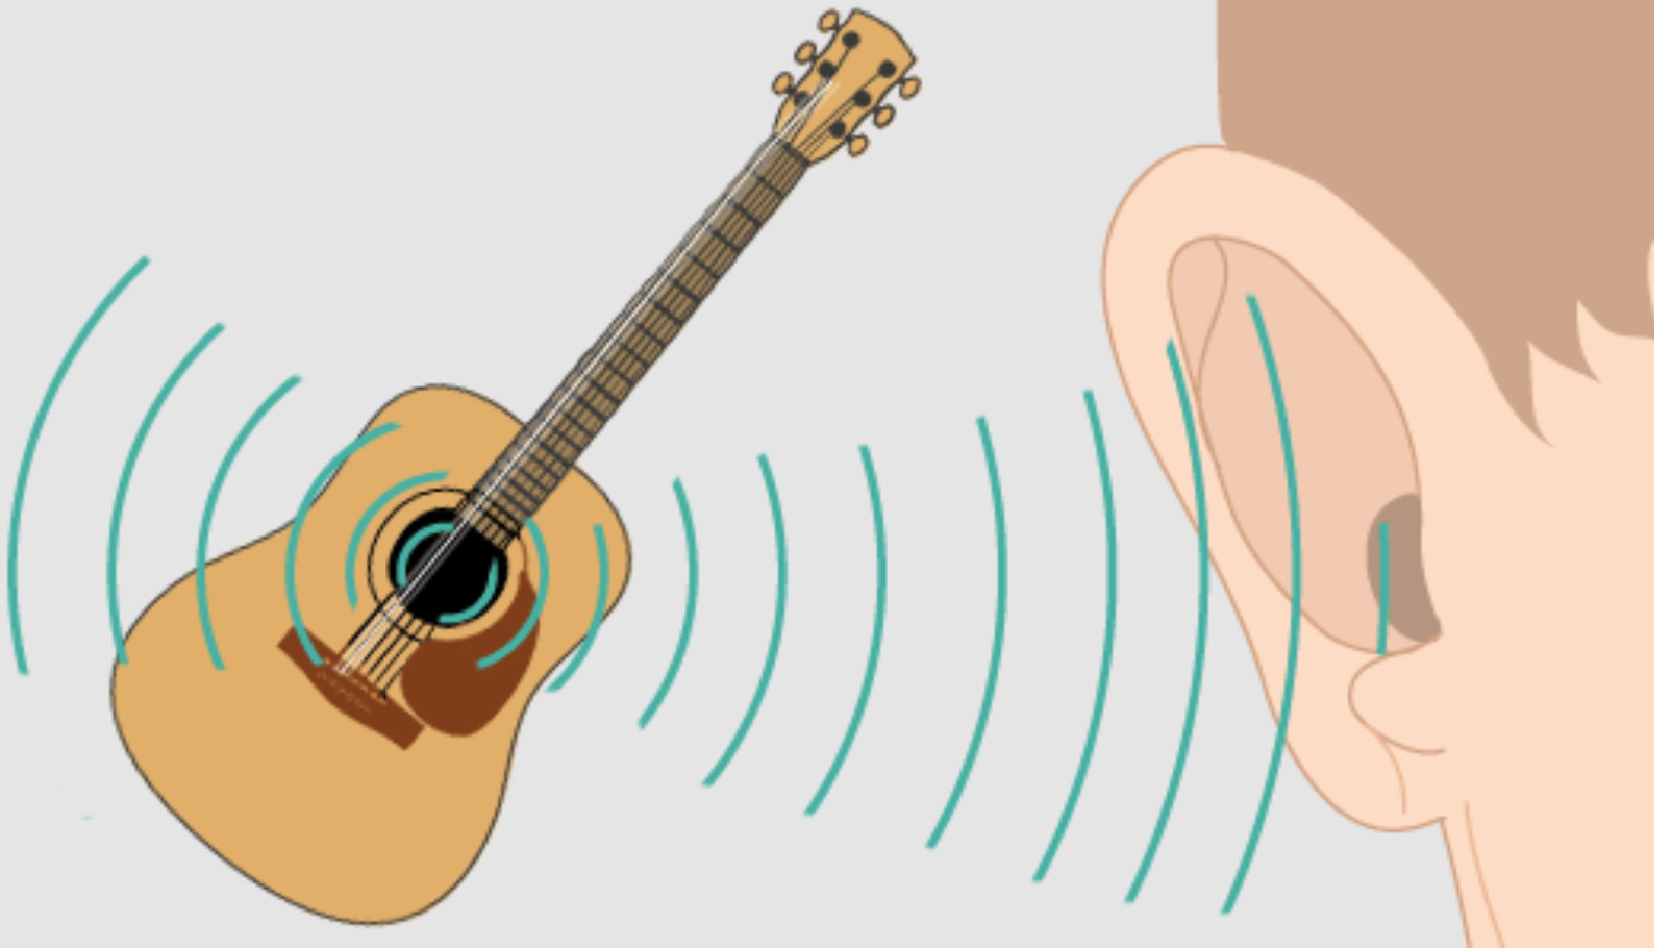
\includegraphics[scale=0.3]{images/transition.pdf}
		\caption{Le signal sonore fait vibrer la membrane tympanique}
		\label{fig:transition}
	\end{center}
\end{figure}

\newpage

%%%%%%%%%%%%%%%%%%%%%%%%%%%%%%%%%%%%%%%%%%%%%%%%%%%%%%%%
% 						                  	PARTIE II         
%%%%%%%%%%%%%%%%%%%%%%%%%%%%%%%%%%%%%%%%%%%%%%%%%%%%%%%%

\section*{Partie II : Modélisation de la membrane tympanique}

Dans cette partie, la propagation d'ondes en deux dimensions est illustrée par une vibration transverse d'une membrane élastique.

\subsection{Modélisation physique d'une membrane circulaire libre fixée sur les bords}

On note $\Omega$ le domaine occupé par la membrane de masse par unité de surface $\rho$ constante. Considérons un petit élément de surface $dxdy$ soumis à des forces de tension $T$  dans les directions $x$ et $y$, une force extérieure de densité surfacique $f(x,y,t)$ et $w(x,y,t)$ la position transversale du point de coordonnées $(x,y)$ à l'instant $t$. D'après la seconde loi de Newton la somme des forces s'exerçant sur $dxdy$ s'écrivent : 
\[
F=\rho  \frac{\partial^2 w}{\partial t^2}(x,y)dxdy
\]
Sachant que la membrane est soumise aux forces suivantes représentées Figure \ref{fig:membrane}, à savoir 4 tensions : $F_1=-Tdy\frac{\partial w}{\partial x}(x,y,t)$, $F_2=Tdy\frac{\partial w}{\partial x}(x+dx,y,t)$, $F_3=-Tdx\frac{\partial w}{\partial y}(x,y,t)$, $F_4=Tdx\frac{\partial w}{\partial y}(x,y+dy,t)$ et une force extérieure $F_5=f(x,y,t)dxdy$, la somme des forces s'écrit : 
\[
F=Tdy\left[\frac{\partial w}{\partial x}(x+dx,y,t)-\frac{\partial w}{\partial x}(x,y,t)\right]+Tdx\left[\frac{\partial w}{\partial y}(x,y+dy,t)-\frac{\partial w}{\partial y}(x,y,t)\right]+f(x,y,t)dxdy
\]

Or les termes entre crochets valent $\dfrac{\partial^2 w}{\partial x^2}$ et $\dfrac{\partial^2 w}{\partial y^2}$ d'où pour $f=0$ la membrane vérifie l'équation 
\[
\rho \dfrac{\partial^2 w}{\partial t^2}=T \Delta w
\]
où $\Delta$ est l'opérateur laplacien définit par 
\[
\Delta w=\dfrac{\partial^2 w}{\partial x^2}+\dfrac{\partial^2 w}{\partial y^2}
\]

\begin{figure}
	\begin{center}
		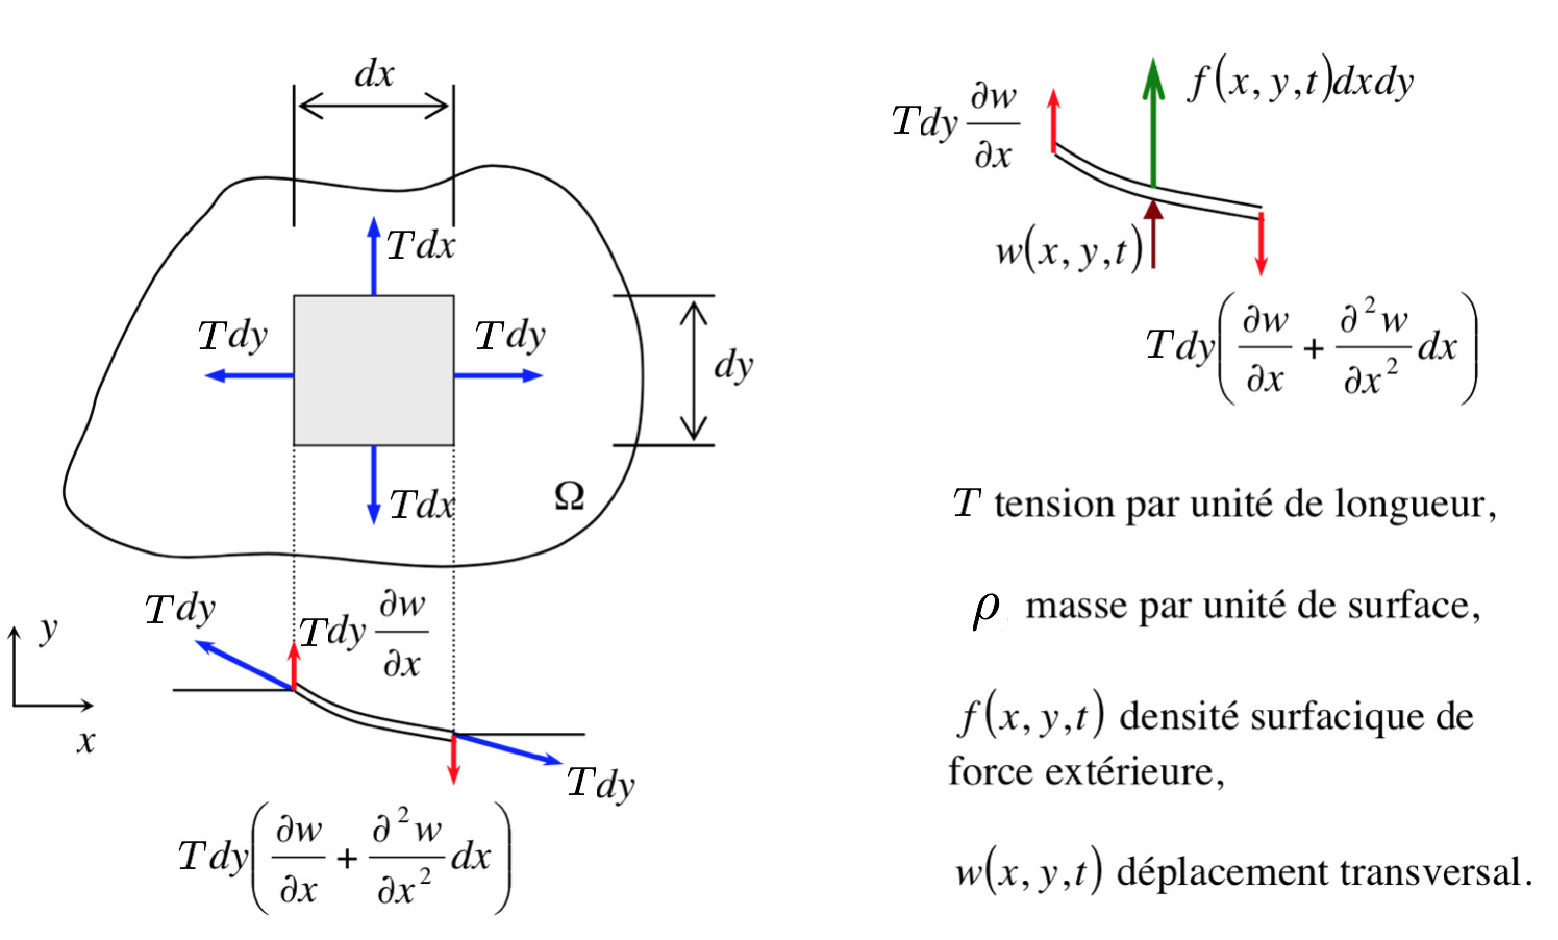
\includegraphics[width=\textwidth]{images/membrane-equation.pdf}
		\caption{Forces de tension s'exerçant aux extrémités d'un élément de surface de la membrane}
		\label{fig:membrane}
	\end{center}
\end{figure}

On cherche à résoudre le problème suivant, trouver $w(x,y,t)$ sur une durée $T_f$ solution de :
\begin{equation}
\left\{
\begin{array}{rl}
\rho \dfrac{\partial^2 w}{\partial t^2} & =  T \Delta w ~\textrm{dans } ~ \Omega_T = \Omega \times (0,T_f)\\ 
w(x,y,t)& =  0 ~\textrm{sur} ~ \Gamma_T=\Gamma \times (0,T_f)\\
w(x,y,0)& = w_0(x,y) ~ \textrm{sur} ~\Omega \\
\dfrac{\partial w(x,y,0)}{\partial t} & = 0 ~\textrm{sur} ~\Omega 
\end{array}
\right.
\label{eq:membranemodel}
\end{equation}

Comme pour la corde de guitare, la membrane est fixée sur le bord circulaire (deuxième équation, condition de type Dirichlet), possède un déplacement initial $w_0(x,y)$ (troisième équation) et une vitesse initiale nulle (quatrième équation). Afin de modéliser la vibration d'une membrane circulaire, il est plus pratique d'utiliser les coordonnées polaires, notamment pour l'écriture des conditions aux bords. On note $a>0$ le rayon de la membrane circulaire : 
\[
\Omega=\{(x,y)\in \R^2, x^2+y^2 \leq a^2\}, \quad \Gamma=\{(x,y)\in \Omega,  x^2+y^2 = a^2\}
\]

Soit $(x,y)$ les coordonnées cartésiennes d'un point de la membrane et $(r,\theta)$ ses coordonnées dans la base polaire on a :
\begin{center}
	\begin{minipage}[l]{.9\linewidth}
	
	\begin{minipage}[l]{.4\linewidth}
	\begin{equation*} 
	\left\{ 
	\begin{array}{rcl}
		x=r\cos(\theta) \\
		y=r\sin(\theta)
	\end{array} 
	\right.
	\end{equation*}
 	\end{minipage}
 et
	\begin{minipage}[r]{.4\linewidth}
	 \begin{equation*} 
	 \left\{ 
	 \begin{array}{rcl}
		r=\sqrt{x^2+y^2} \\
		\theta=\arctan(\frac{y}{x})
	\end{array} 
	\right.
	\end{equation*}
	 \end{minipage}

	 \end{minipage}
\end{center}

avec $r \in[0,a]$ et $\theta  \in [0,2\pi]$. On peut alors calculer les dérivées partielles de $u$ dans la base polaire $(r,\theta)$ en utilisant les formules suivantes :
\[
\dfrac{\partial w}{\partial x}=\left(\dfrac{\partial w}{\partial r}\right)\left(\dfrac{\partial r}{\partial x}\right)+\left(\dfrac{\partial w}{\partial \theta}\right)\left(\dfrac{\partial \theta}{\partial x}\right)
\]
\[
\dfrac{\partial w}{\partial y}=\left(\dfrac{\partial w}{\partial r}\right)\left(\dfrac{\partial r}{\partial y}\right)+\left(\dfrac{\partial w}{\partial \theta}\right)\left(\dfrac{\partial \theta}{\partial y}\right)
\]

On introduit les variables adimensionnées suivantes 
\[
\eta=\dfrac{r}{a},\tau=\dfrac{ct}{a}
\]
où $c=\sqrt{\frac{T}{\rho}}$ représente la vitesse de propagation  de l'onde.\\ 

%--- Question 8 ---%

\begin{mdframed}[style=exampledefault]
\question Montrer que le problème (\ref{eq:membranemodel}) devient l'EDP suivante en coordonnées polaires :\\

Trouver $w(\eta,\theta,\tau)$ solution de :
\begin{equation}
	\left\{
	\begin{array}{rl}
		 \dfrac{\partial^2 w}{\partial \tau^2} & =   \dfrac{\partial^2 w}{\partial \eta^2}+\dfrac{1}
		 {\eta^2}\dfrac{\partial^2 w}{\partial \theta^2}+\dfrac{1}{\eta}\dfrac{\partial w}{\partial \eta},\;\eta\in[0,1],\;		\theta\in[0,2\pi],\;\tau>0\\
		w(1,\theta,\tau)& = 0  \\
		w(\eta,\theta,0)& = w_0(\eta \cos(\theta),\eta \sin (\theta)) \\
		\dfrac{\partial w(\eta,\theta,0)}{\partial \tau} & = 0
	\end{array}
	\right.
	\label{eq:polarmodel}
\end{equation}

On ajoute à cette équation une condition limite nécessaire  en $\eta=0$ :
\[
w(0,\theta,\tau)=w^0
\]
\end{mdframed}

%--- Fin Question 8 ---%

Le laplacien s'exprime en coordonnées polaires de la manière suivante :

$$
\Delta w = \frac{1}{r} \frac{\partial}{\partial r} (r \frac{\partial w}{\partial r}) +
\frac{1}{r^2} \frac{\partial^2 w}{\partial \theta^2} =
\frac{\partial^2 w}{\partial r^2} + \frac{1}{r} \frac{\partial w}{\partial r} + \frac{1}{r^2} \frac{\partial^2 w}{\partial \theta^2}
$$

En effet :

TODO
http://www.cafepedagogique.net/communautes/MarcCourbot/Documents/TRAVAUX%20SUR%20LE%20LAPLACIEN/2D%20-%20LAPLACIEN.pdf

Or :

$$
\left\{\begin{aligned}
    \frac{\partial w}{\partial r} &= \frac{1}{a} \frac{\partial w}{\partial \eta} \\
    \frac{\partial^2 w}{\partial r^2} &= \frac{1}{a^2} \frac{\partial^2 w}{\partial \eta^2} \\
    \frac{\partial^2 w}{\partial t^2} &= \frac{c^2}{a^2} \frac{\partial^2 w}{\partial \tau^2} \\
                                      &= \frac{T}{\rho a^2} \frac{\partial^2 w}{\partial \tau^2}
\end{aligned}\right.
$$

Donc :

$$
\begin{aligned}
  \rho \dfrac{\partial^2 w}{\partial t^2} = T \Delta w
  &\Leftrightarrow
  \rho \frac{T}{\rho a^2} \frac{\partial^2 w}{\partial \tau^2} = T(\frac{1}{a^2} \frac{\partial^2 w}{\partial \eta^2} + \frac{1}{a\eta} \frac{1}{a} \frac{\partial w}{\partial \eta} + \frac{1}{\eta^2 a^2} \frac{\partial^2 w}{\partial \theta^2}) \\
  &\Leftrightarrow
  \frac{\partial^2 w}{\partial \tau^2} = \frac{\partial^2 w}{\partial \eta^2} + \frac{1}{\eta} \frac{\partial w}{\partial \eta} + \frac{1}{\eta^2} \frac{\partial^2 w}{\partial \theta^2}
\end{aligned}
$$

\subsection{Discrétisation polaire de la surface 2D par un schéma explicite }
Le but de cette partie est de discrétiser l'équation des ondes dans la base polaire (\ref{eq:polarmodel}) en utilisant un schéma explicite. Pour cela considérons dans un premier temps une discrétisation de $\Omega $ suivant une grille cartésienne $[0,N_x]\times [0,N_y]$ de pas uniforme $dx$, $dy$, formée par des points de coordonnées $(x_i,y_j)$ tel que :
\begin{equation*}{}
	\left\{
	\begin{array}{rl}
		x_i &=i dx,\quad 0\leq i \leq N_x \\
		y_j &=j dy,\quad  0\leq j \leq N_y \\
 		dx & =\frac{1}{N_x+1}\\
		 dy &=\frac{1}{N_y+1}\\
	\end{array}
	\right.
\end{equation*}
On note $dt$ le pas de temps et on approche la solution $w(x_i,y_j,ndt)$ par $w_{ij}^{n}$. Le laplacien est discrétisé  par un schéma centré d'ordre deux  et on utilise un schéma explicite d'ordre deux en temps. L'ordre de ces schémas peut être vérifié en utilisant un développement de Taylor. Le schéma explicite obtenue pour l'équation des ondes (\ref{eq:membranemodel}) est :

\begin{equation}
	\left\{
	\begin{array}{rl}
		\dfrac{w_{ij}^{n+1}-2w_{ij}^{n}+w_{ij}^{n-1}}{dt^{2}}=c^2\dfrac{w_{i+1,j}^{n}-2w_{i,j}^{n}+w_{i-1,j}^{n}}
		{dx^{2}}+c^2\dfrac{w_{i,j+1}^{n}-2w_{i,j}^{n}+w_{i,j-1}^{n}}{dy^{2}}
	\end{array}
	\right.
	\label{eq:diffcartesiennes}
\end{equation}

%--- Question 9 ---%

\begin{mdframed}[style=exampledefault]
\question En utilisant un développement de Taylor  et le  schéma explicite (\ref{eq:diffcartesiennes}) écrire les conditions initiales et les conditions limites de l'équation (\ref{eq:membranemodel}) obtenues pour $w_{i,j}^0,w_{i,j}^1$ sur la grille cartésienne.
\end{mdframed}

%--- Fin Question 9 ---%

%--- Question 10 ---%

\begin{mdframed}[style=exampledefault]
\question On note maintenant $w_{ij}^{n}=w(id\eta,jd\theta,nd\tau)$ les valeurs aux noeuds de la grille polaire représentée Figure \ref{fig:polaire}. Ecrire le schéma explicite de l'équation (\ref{eq:polarmodel}).
\end{mdframed}

%--- Fin Question 10 ---%

\begin{figure}
	\begin{center}
		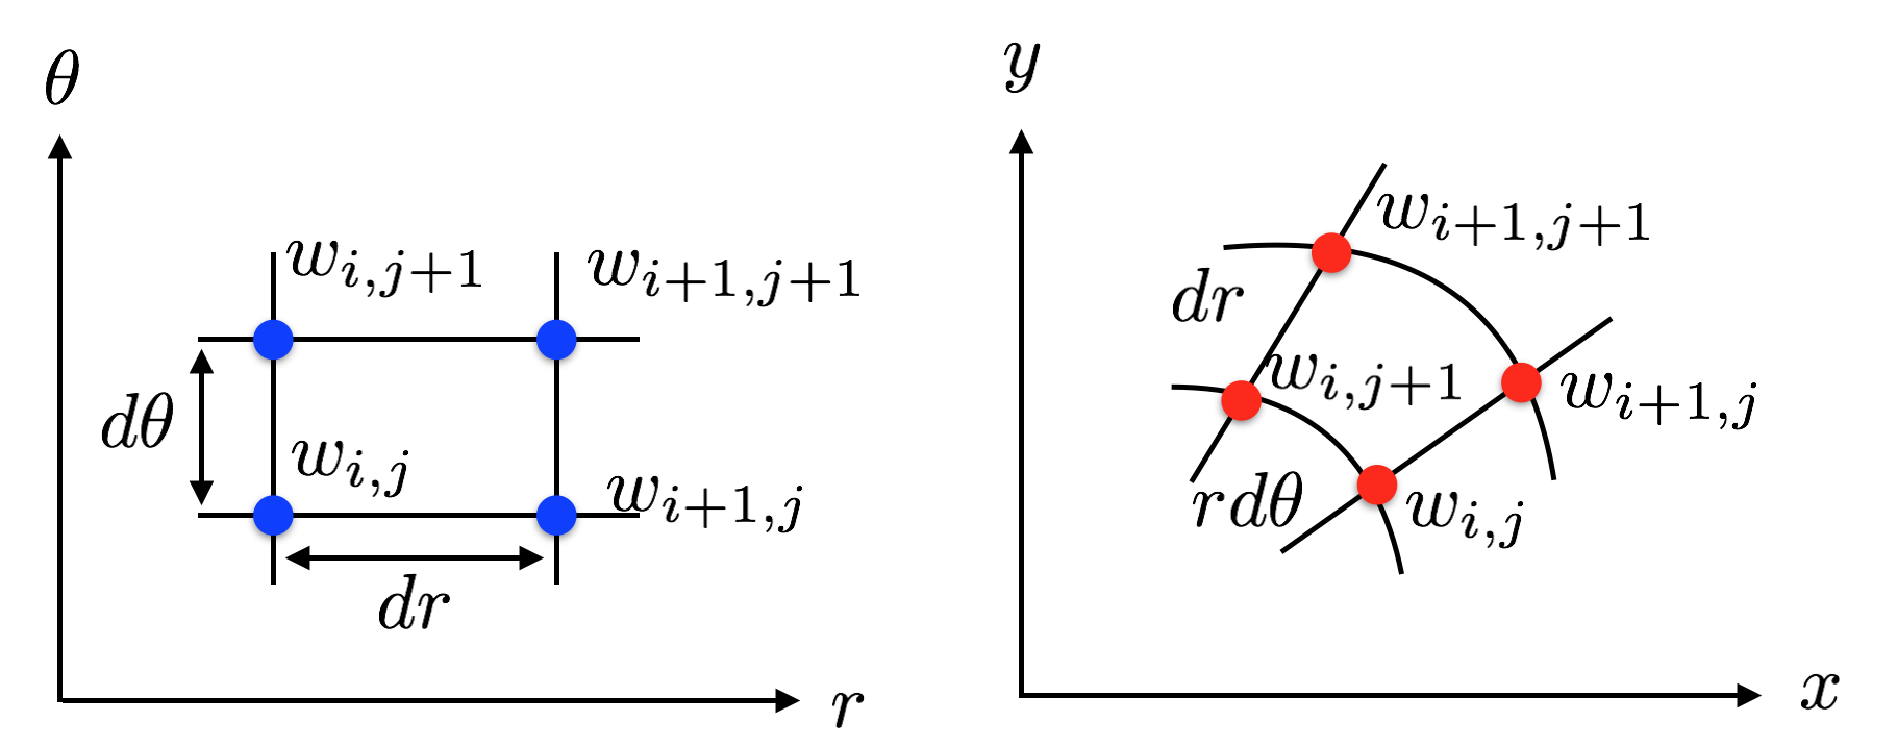
\includegraphics[width=0.8\textwidth]{images/polaire.pdf}
		\caption{Grille polaire}
		\label{fig:polaire}
	\end{center}
\end{figure}

On montre qu'une condition limite en $\eta=0$ sur la grille polaire se détermine en utilisant le schéma explicite en coordonnées cartésiennes (\ref{eq:diffcartesiennes}), on obtient :
\[
\dfrac{w_0^{n+1}-2 w_0^{n}+ w_{0}^{n-1}}{d\tau^2}=\dfrac{4}{d \eta^2}\left(\frac{1}{N_\theta} \sum_{j=1}^{N_\theta} w_{1,j}^n-w_{0}^{n}\right)
\]

\subsection{Stabilité et précision du schéma}

\subsubsection{Etude de la stabilité}
Commencons par une étude de la stabilité du schéma explicite (10), pour cela on remplace $w_{i,j}^{n}$ dans l'équation discrétisée, par une solution décomposée en modes de fourier: 
\[
W_{p_{i,j}}^{n}=\phi^n e^{i\alpha_1(idx)}e^{i\alpha_2(jdy)}
\]

%--- Question 11 ---%

\begin{mdframed}[style=exampledefault]
\question Soit $J=\dfrac{\phi^{n+1}}{\phi^n}$ le coefficient d'amplification, montrer que $J$ vérifie l'équation du second degré suivante : 
\[
J^2+\gamma J+1=0
\]
avec 
\[
\gamma=-2+2c^2\dfrac{dt^2}{dx^2}(1-\cos(\alpha_1dx))+2c^2\dfrac{dt^2}{dy^2}(1-\cos(\alpha_2dy))
\]
En admettant que le schéma explicite (\ref{eq:membranemodel}) est stable sous la condition 
\[
\vert J \vert \leq 1
\]
en déduire que cette condition de stabilité s'écrit aussi :
\[
c^2\left(\dfrac{dt^2}{dx^2}+\dfrac{dt^2}{dy^2}\right)\leq 1
\]
\end{mdframed}

%--- Fin Question 11 ---%

Ainsi en posant $\displaystyle h=\dfrac{dxdy}{\sqrt{dx^2+dy^2}}$ on obtient la condition de courant : 
\begin{equation}
	\begin{array}{l}
		CFL=c\dfrac{dt}{h} \leq 1~[\textrm{Cartésien}] \\ \\
		\displaystyle CFL=\frac{d \tau}{d \eta d \theta}\leq 1~[\textrm{Polaire}]
	\end{array}
	\label{eq:CFL}
\end{equation}

\subsubsection{Etude de la consistance}
On souhaite étudier la précision du schéma explicite (\ref{eq:diffcartesiennes}) en coordonnées cartésiennes.

%--- Question 12 ---%

\begin{mdframed}[style=exampledefault]
\question En développant $w_{i,j}^{n+1},w_{i,j}^{n},w_{i,j}^{n-1}$ par un développement de Taylor montrer que le schéma est d'ordre 2 en temps \textit{i.e} l'erreur de troncature est en $o(dt^2)$.\\
En suivant le même principe avec les termes en espace $w_{i+1,j}^{n},w_{i-1,j}^{n},w_{i,j-1}^{n},w_{i,j}^{n},w_{i,j+1}^{n}$ montrer que l'erreur de troncature est en $o (dx^2,dy^2)$.\\
Ecrire alors l'erreur de troncature $E_t$ du schéma et en déduire que le schéma est d'ordre deux en temps et en espace. Ainsi le schéma explicite (\ref{eq:diffcartesiennes}) est consistant 
\[
\lim_{(dt,dx,dy)\longrightarrow 0} E_t=0
\]
\end{mdframed}

%--- Fin Question 12 ---%

\subsection{Solutions analytiques }
On cherche une solution de notre équation d'onde polaire sous la forme :
\[
w(\eta,\theta,\tau)=F(\eta,\theta)\cos(\omega \tau)
\]
avec $\omega$ la fréquence de vibration de l'onde et $F$ l'amplitude.

%--- Question 13 ---%

\begin{mdframed}[style=exampledefault]
\question Ecrire l'équation différentielle vérifiée par l'amplitude $F$.\\

La condition limite $F(1,0)=0$ nous permet de décomposer l'amplitude $F(\eta,\theta)$ sous la forme :
\[
F(\eta,\theta)=\sum_n F_n(\eta)\cos(n\theta)
\]
Montrer que chaque $F_n$ vérifie l'équation de Bessel suivante, avec  $\alpha=\omega\eta$ :
\[
\frac{d^2 F_n}{d\alpha^2}+\frac{1}{\alpha}\frac{dF_n}{d\alpha}+\left(1-\frac{n^2}{\alpha^2}\right)F_n=0
\]
\end{mdframed}

%--- Fin Question 13 ---%

\begin{table}
	\begin{center}
		\begin{tabular}{|c|c|c|c|c|c|}
			\hline
			$\lambda_{n,m}$&$m=1$  &$m=2$ & $m=3$ &$ m=4$&$m=5$\\
			\hline
			$n=0$&2.40483&$5.52008$&$8.65373$&$11.79153$&$14.93092$\\
			\hline
			$n=1$&$3.83171$&$7.01559$&$10.17347$&$13.32369$&$16.47063$\\
			\hline
			$n=2$&$5.13562$&$8.41724$&$11.61984$&$14.79595$&$17.95982$\\
			\hline
			$n=3$&$6.38016$&$9.76102$&$13.01520$&$16.22347$&$19.40942$\\
			\hline
			$n=4$&$7.58834$&$11.06471$&$14.37254$&$17.61597$&$20.82693$\\
			\hline
		\end{tabular}
		\caption{Valeurs des cinq premiers zéros des fonctions de Bessel $J_n$.}
 	\end{center}
\end{table}

Les solutions de cette équation sont les fonctions de Bessel. Par ailleurs, c'est une équation du second ordre il existe donc deux solutions linéairement indépendantes. La solution est donc de la forme :
\[
F_n(\eta)=d_nJ_n(\eta)+e_nY_n(\eta)
\]
avec les fonctions de Bessel d'ordre $n$ de première et deuxième espèce suivantes :
\[
J_n(\eta)=\left(\dfrac{\eta}{2}\right)^n\sum_{m=0}^{\infty} \dfrac{(-\eta^2/4)^m}{m!\int_0^{\infty}e^{-t}t^{n+m}dt}
\]
\[
Y_n(\eta)=\dfrac{J_n(\eta)\cos(n\pi)-J_{-n}(\eta)}{\sin(n\pi)}
\]
Or les fonctions $Y_n(x)$ divergent au centre de la membrane $(\eta\rightarrow 0)$ donc $e_n=0$
ainsi la solution analytique de l'équation (\ref{eq:polarmodel}) est donnée par :
\[
w(\eta,\theta,\tau)=\cos(\omega \tau)\sum_n d_nJ_n(\omega\eta)\cos(n\theta)
\]
On sélectionne les fréquences en utilisant les conditions limites. Par exemple, dans le cas $n=0$, 
\[
w(\eta,\theta,\tau)=\cos(\omega \tau) d_0J_0(\omega \eta)
\]
ainsi $\omega$ décrit les zéros de $J_0$ puisque la condition aux bords est $w(1,\theta,\tau)=0$. Si on note $\lambda_{m,0}$ la suite de ces zéros, on obtient les fréquences propres de vibration de la membrane :
\[
\eta_{m,0}=\dfrac{\lambda_{m,0}}{2\pi a} \sqrt{\frac{T}{\rho}}
\]
En notant $\lambda_{m,n}$ la $m$-ième racine de $J_n$, on obtient de même 
\[
\eta_{m,n}=\dfrac{\lambda_{m,n}}{2\pi a} \sqrt{\frac{T}{\rho}}
\]

Les valeurs numériques des racines des fonctions de Bessel $J_n$ sont fournies Table 1. Il en découle que les fréquences propres $\eta_{m,n}$ ne sont pas des multiples de la fréquence fondamentale. Par conséquent le son produit par la membrane n'est pas harmonique.

\newpage 

\subsection{Code scilab du schéma explicite et analyse des résultats}

Afin de résoudre numériquement le schéma explicite en coordonnées polaires, on définit $w_{ij}^n$ comme un tableau de taille $(N_\eta)\times(N_\theta+1)$ avec :
\[
\eta=id\eta ,\;i=1,..,N_\eta
\]
\[
\theta=jd\theta ,\;j=1,..,N_\theta+1
\]
On pose des conditions périodiques en $\theta$ :
\[
w(\eta,\theta,\tau)=w(\eta,\theta+2\pi,\tau)
\]

%--- Question 14 ---%

\begin{mdframed}[style=exampledefault]
\question On prend la condition initiale suivante:
\begin{equation}
	w(\eta,\theta,0)=J_0(\lambda_{0,3}\eta)
	\label{eq:condinit}
\end{equation}
avec $\lambda_{0,3}=8.65373$, la valeur approchée de la troisième valeur propre de $J_0$ correspondant à la fréquence du mode (0,3). De cette façon on a $d_0=1$.\\

Ecrire un programme scilab qui résout numériquement le schéma explicite en coordonnées polaires de l'équation (\ref{eq:polarmodel}) avec les données suivantes : 
\[
\begin{array}{ll}
	\bullet & N_\theta=80 \\ 
	\bullet & N_\eta=40 \\ 
	\bullet & CFL=0.5 \\ 
	\bullet & c=1
\end{array}
\]
Utilisez la fonction $besselj$ de Scilab pour implémenter la condition initiale (voir Figure \ref{fig:bessel}).\\
Créez une animation représentant les vibrations de la membrane à différents instants $w^n$.
\end{mdframed}

%--- Fin Question 14 ---%

\begin{figure}[H]
	\begin{center}
		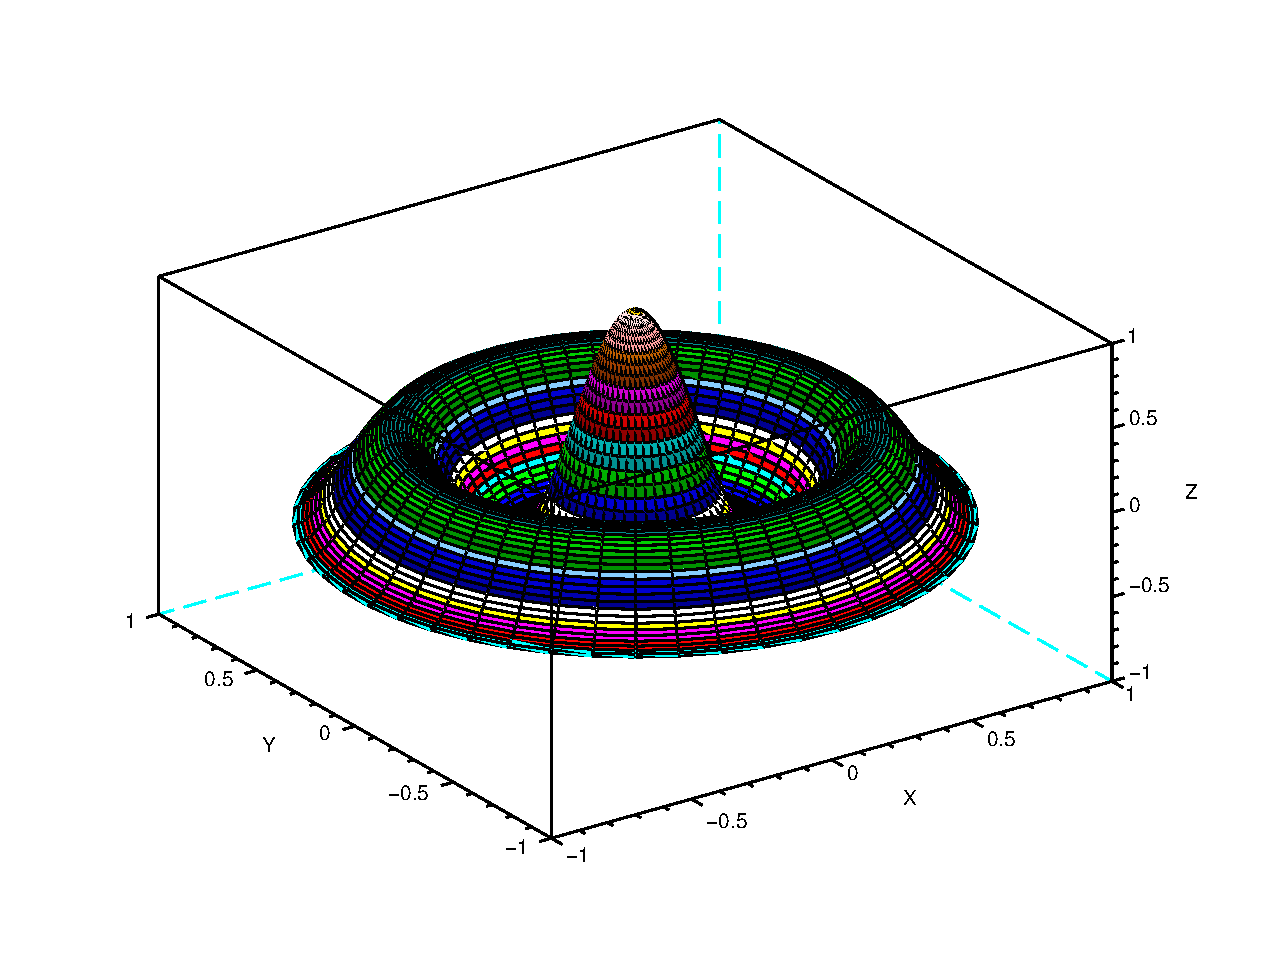
\includegraphics[scale=0.4]{images/joinitial.pdf}
		\caption{Etat initial de la membrane}
		\label{fig:bessel}
	\end{center}
\end{figure}

%--- Question 15 ---%

\begin{mdframed}[style=exampledefault]
\question La solution analytique correspondant à la condition initiale (\ref{eq:condinit}) est :
\[
w_{ex}(\eta,\theta,\tau)=\cos(\lambda_{0,3} \tau)J_0(\lambda_{0,3}\eta)
\]
Comparer visuellement les deux solutions (analytique $w_{ex}$ et numérique $w_{num}$) en vérifiant qu'elles possèdent bien le même comportement.
Tracez l'erreur relative en $\eta=0$ en fonction du temps pour   différentes valeurs de la CFL. 
Qu'observez-vous ?
\end{mdframed}

%--- Fin Question 15 ---%

%--- Question 16 ---%

\begin{mdframed}[style=exampledefault]
\question On fixe la CFL à 0.8. Tracez l'erreur relative globale $\|w_{ex}-w_{num}\|_{\infty}$ pour les grilles de taille ($N_\theta=80$, $N_\eta=40$), ($N_\theta=40$,$N_\eta=20$) et ($N_\theta=160$,$N_\eta=80$).\\
Comparez l'erreur relative obtenue pour les trois différentes grilles et en déduire que le schéma est d'ordre deux en espace.
\end{mdframed}

%--- Fin Question 16 ---%

%--- Question 17 ---%

\begin{mdframed}[style=exampledefault]
\question On souhaite à présent représenter le mode (1,1) pour cela on introduit la condition initiale suivante:
\[
w(\eta,\theta,0)=\dfrac{J_1(\lambda_{1,1}\eta)\cos(\theta)}{2}
\]
Créez une animation de la vibration de la membrane à différents instants.
Dans le lien suivant 
\begin{center}
	\url{http://www.acs.psu.edu/drussell/demos/membranecircle/circle.html}
\end{center} 
différents modes de vibration de la membrane sont représentés.
Vous pouvez ainsi comparer  vos résultats.
\end{mdframed}

\subsection{Pour aller plus loin}

Nous avons modéliser et simuler le comportement d'une \enquote{membrane idéale}, tout en contrôlant la précision du schéma et sa stabilité. On pourrait reprendre ce travail pour un modèle de membrane plus sophistiqué (et donc plus réel), qui comme pour le modèle avancé qu'on a étudié pour la corde de guitare, prendrait en compte la physique du matériel composant la membrane et les différents termes d'amortissements. De cette façon on peut alors modéliser un instrument de percussion comme un tambour, une caisse claire ou une cymbale, et en simuler le son émis. \\

Enfin on vous propose de découvrir un phénomène vibratoire amusant (après l'effort, le réconfort). Il s'agit des motifs de Chladni, que vous seriez capable d'expliquer en caractérisant les lignes nodales des différents modes de la membrane, c'est-à-dire les points de sa surface qui ne bougent pas au cours du temps $w=0$. Ainsi si on place de la semoule sur la membrane en vibration, les grains se regroupent au niveau des lignes nodales. Voyez par vous-même :

\begin{center}
	\url{https://www.youtube.com/watch?v=1yaqUI4b974}
\end{center}

\newpage

\section*{Annexe : aide scilab pour les animations et le son}

\hspace{0.5cm} $\blacksquare$ \textbf{Produire un son stéréo avec Scilab}\\

C'est très simple, il suffit d'appeler la commande 
\[
playsnd(out(1:size(out,1)),SR)
\]
qui va envoyer chacune des 2 composantes de $out$ aux 2 hauts parleurs qui vont reproduire les vibrations enregistrées en tenant compte du taux l'échantillonnage $SR$.\\

Vous pouvez enregistrer les sons pour mieux les comparer via la commande 
\[
savewave("son.wav",out(1:size(out,1)),SR)
\]

\hspace{0.5cm} $\blacksquare$ \textbf{Créer une animation avec Scilab}\\

Là encore ce n'est pas bien compliqué, il suffit d'utiliser les commandes $drawlater$ et $drawnow$ :

\begin{lstlisting}[frame=single,caption=Création d'une animation dans une boucle]  
start
for n=1:fin
drawlater;
// calcul effectif
clf();
plot(...);
drawnow;
end
\end{lstlisting}

Pensez à garder une fenêtre d'affichage fixe tout au long de l'animation, en ajoutant après $plot$ : 

\begin{lstlisting}[frame=single,caption=Fixer les dimensions du repère courant]  
start
a=gca();
a.data_bounds=[xmin,ymin ; xmax,ymax];
\end{lstlisting}

\textit{Remarques} : pour afficher simultanément l'animation de la corde $\ub^n$ et les 2 onde sonores $out(:,1)$ et $out(:,2)$ utilisez la commande $subplot$. Pour \enquote{accélerer} une animation, il suffit de ne pas afficher tous les incréments de boucle, par exemple en utilisant la fonction $modulo$.\\

\hspace{0.5cm} $\blacksquare$ \textbf{Enregistrer les images de l'animation et créer un gif animé}\\

Pour enregistrer les images, déclarer en tête de fichier $driver("Rec")$ et ajouter dans la boucle

\begin{lstlisting}[frame=single,caption=Enregistrer des images sous Scilab]  
start
nom_image='image_'+string(n)+'.gif'; 
xs2gif(winnum($),nom_image);
\end{lstlisting}

Enfin on créé le .gif animé à l'aide de la commande d'ImageMagick suivante dans un terminal : 
\begin{center}
	\begin{verbatim}
		convert -delay 10 -loop 0 image_*.gif animation.gif
	\end{verbatim}
\end{center}
 
\end{document}

% Fin du document LaTeX
